%% Journal of Scientific Computing (Springer): svjour3 class, option smallextended
%% as required by the journal's submission guidelines. The class files
%% svjour3.cls, svglov3.clo and the bibliography style spmpsci.bst (Springer
%% LaTeX package, numbered references) are included in this folder.
\RequirePackage{fix-cm}
\documentclass[smallextended]{svjour3}
\smartqed

% Show the pages on the journal's trim size, 155 mm x 235 mm (the page size of
% published JSC articles), instead of A4. The class option smallextended sets
% the text block (119 mm x 195 mm) for this format but prints it at the top left
% of an A4 sheet, which leaves wide empty margins. Only the paper size and the
% position of the text block change; line and page breaks are the same. Remove
% these lines to get the class's A4 output.
\setlength{\paperwidth}{155mm}
\setlength{\paperheight}{235mm}
\setlength{\hoffset}{\dimexpr(\paperwidth-\textwidth)/2-1in\relax}
\setlength{\voffset}{-34pt}
\AtBeginDocument{\setlength{\pdfpagewidth}{\paperwidth}\setlength{\pdfpageheight}{\paperheight}}

% ---------------------------------------------------------------------------
% Version of paper/main_light.tex for submission to the Journal of Scientific
% Computing. paper/ holds the preprint archived on Zenodo; edit this file for the
% journal version.
% Main paper: method and results written as prose, without definitions,
% theorems or proofs. The mathematical results with proofs are collected in
% the separate addendum (supplementary material). Results: HyperCloudCore 0.7.8.
% ---------------------------------------------------------------------------

% ---------------------------------------------------------------------------
% Packages
% ---------------------------------------------------------------------------
\usepackage[utf8]{inputenc}
\usepackage{amsmath,amssymb,mathtools}
\usepackage{bm}
\usepackage{graphicx}
\usepackage{booktabs}
\usepackage{adjustbox}
\usepackage{array}
\usepackage{xcolor}
\usepackage{tikz}
\usetikzlibrary{arrows.meta,calc,decorations.pathreplacing}
\usepackage{enumitem}
\usepackage[labelfont=bf]{caption}
\usepackage{subcaption}
\usepackage[numbers,square,sort&compress]{natbib}
\usepackage{microtype}
\usepackage[section]{placeins}% floats are output before the next section starts
\usepackage[colorlinks=true,linkcolor=blue!50!black,citecolor=green!35!black,urlcolor=blue!60!black]{hyperref}
% svjour3 + amsmath leave \cl@chapter self-referential, which makes cleveref
% loop (TeX capacity exceeded); the paper has no chapters, so reset it.
\makeatletter\let\cl@chapter\relax\makeatother
\usepackage[capitalise,nameinlink]{cleveref}

% Springer style: "Fig. 1" (bold label, no punctuation after the number),
% sub-figures (a), (b), ...
\captionsetup{font=small,labelsep=space}
\captionsetup[sub]{labelformat=parens,labelsep=space,labelfont=normalfont}
\setlist{itemsep=2pt,topsep=4pt}

% Full DOI links in the reference list, as required by the journal.
\newcommand{\doi}[1]{\url{https://doi.org/#1}}

% Placeholders for information the authors still have to supply.
\newcommand{\TODO}[1]{\textcolor{red}{[TODO: #1]}}

% Float placement: allow larger floats at the top of text pages and fuller float
% pages, so that figures and tables stay close to the text that cites them.
\renewcommand{\topfraction}{0.85}
\renewcommand{\bottomfraction}{0.6}
\renewcommand{\textfraction}{0.12}
\renewcommand{\floatpagefraction}{0.75}
\setcounter{topnumber}{3}
\setcounter{bottomnumber}{2}
\setcounter{totalnumber}{5}

% ---------------------------------------------------------------------------
% Macros
% ---------------------------------------------------------------------------
\numberwithin{equation}{section}

\crefname{figure}{Fig.}{Figs.}
\Crefname{figure}{Fig.}{Figs.}

\newcommand{\R}{\mathbb{R}}
\newcommand{\dd}{\mathrm{d}}
\newcommand{\nb}{\nu}
\newcommand{\cnb}{\bar\nu}
\newcommand{\Ad}{\mathcal{G}}
\newcommand{\Lop}{\mathcal{L}}
\newcommand{\Fs}{F^{*}}
\newcommand{\ptil}{\tilde p}
\newcommand{\Ntil}{\tilde N}
\newcommand{\sgn}{\operatorname{sign}}
\newcommand{\ord}[2]{k_{#1\to #2}}
\newcommand{\qdiv}{q}
\newcommand{\CFL}{\mathrm{CFL}}

\definecolor{lowc}{RGB}{200,30,30}
\definecolor{highc}{RGB}{170,170,170}

\journalname{Journal of Scientific Computing}

% ---------------------------------------------------------------------------
\begin{document}

\title{High-order meshfree MUSCL schemes with a~posteriori order detection for hyperbolic systems on scattered point clouds}
\titlerunning{Meshfree MUSCL schemes with a~posteriori order detection}

\author{Pascal Jung \and Klaas Willems \and Axel Klar}
\authorrunning{P. Jung, K. Willems, A. Klar}

\institute{P. Jung \TODO{corresponding author? confirm} \at
  Faculty of Mathematics, RPTU Kaiserslautern-Landau, Kaiserslautern, Germany\\
  \email{\TODO{institutional e-mail of the corresponding author}}\\
  ORCID: \TODO{0000-0000-0000-0000}
  \and
  K. Willems \at
  Faculty of Mathematics, RPTU Kaiserslautern-Landau, Kaiserslautern, Germany\\
  Department of Computer Science, KU Leuven, Leuven, Belgium\\
  ORCID: \TODO{0000-0000-0000-0000}
  \and
  A. Klar \at
  Faculty of Mathematics, RPTU Kaiserslautern-Landau, Kaiserslautern, Germany\\
  ORCID: \TODO{0000-0000-0000-0000}
}

\date{Received: date / Accepted: date}

\maketitle

\begin{abstract}
We present meshfree monotone upstream-centred schemes for conservation laws (MUSCL) of arbitrary design order $k$ for hyperbolic systems on scattered point clouds. Moving least-squares (MLS) reconstructions of degree $k-1$ are evaluated at midpoints between neighbouring particles, jumps are resolved by approximate Riemann solvers, and the interface fluxes are differentiated by an MLS derivative operator whose weights sum to zero. The scheme is exact for polynomial solutions of linear problems, is consistent of order $k$ on periodic Cartesian lattices, and its conservation error is the lack of antisymmetry of the derivative weights. Orienting the dissipation of the Rusanov flux by the signs of the derivative weights keeps density and pressure positive in the first-order fallback for derivative operators of any degree. Discontinuities are treated by slope limiters or a per-particle multi-dimensional optimal order detection (MOOD) procedure within strong-stability-preserving Runge--Kutta methods; as the fallback is positive, the degree of the derivative operator can stay fixed while MOOD lowers only the degree of the reconstructions. Numerical experiments confirm the design orders up to five for smooth solutions on regular and perturbed clouds and show that, with a degree-one derivative operator, the conservation defect at moving shocks decreases under refinement. A two-dimensional Riemann problem and the double Mach reflection are computed robustly with positive density and pressure.
\keywords{Meshfree methods \and Moving least squares \and MUSCL \and MOOD \and A~posteriori limiting \and Compressible Euler equations}
\subclass{65M06 \and 65M08 \and 65M12 \and 35L65 \and 76M28}
\end{abstract}

% ===========================================================================
\section{Introduction}\label{sec:intro}
% ===========================================================================

Hyperbolic systems of conservation laws describe the transport of mass, momentum and energy in compressible flows and many other applications. Their solutions develop discontinuities in finite time, and robust high-resolution discretizations are assembled from a few well-understood ingredients: a conservative flux form, upwinding through exact or approximate Riemann solvers, high-order reconstructions, and a mechanism that suppresses spurious oscillations at discontinuities \cite{vanLeer1979,Harten1987,Shu1998,Toro2009}. In finite volume (FV) and discontinuous Galerkin methods all of these ingredients rest on a mesh: the faces of the control volumes carry the numerical fluxes, the telescoping sum of the fluxes gives discrete conservation, and the cells define the stencils of the reconstruction.

Meshfree methods replace the mesh by a cloud of points, which we call particles, and approximate derivatives from local neighbourhoods. Generalized finite difference methods (GFDM) \cite{Jensen1972,Perrone1975} approximate derivatives from Taylor expansions on local stars of points; since Liszka and Orkisz \cite{Liszka1980} they use weighted least-squares fits of local polynomials \cite{Benito2001,Benito2007}, as do the finite pointset method \cite{Tiwari2003} and moving least-squares (MLS) approximations \cite{Lancaster1981,Levin1998}; see \cite{Belytschko1996,Nguyen2008} for reviews, \cite{Seibold2006} for stencil properties and \cite{Clain2024} for very high-order variants. Since a point cloud needs no connectivity, meshfree methods are attractive for complex and moving geometries, where generating and maintaining a mesh dominates the cost of a simulation.

For hyperbolic problems the mesh-based ingredients do not carry over directly. Central meshfree differentiation is unstable for advection on irregular clouds and requires upwinding or artificial dissipation \cite{FornbergLehto2011,Willems2025}. Shocks require non-oscillatory and positivity-preserving mechanisms that work on irregular and overlapping stencils. And without faces there is no telescoping sum of fluxes, so discrete conservation is not automatic; convergent conservative schemes converge to weak solutions \cite{LaxWendroff1960}, whereas non-conservative schemes may converge to discontinuities that move with wrong speeds \cite{HouLeFloch1994}.

Several lines of work address these issues. Kinetic upwinding on least-squares stencils leads to the least-squares kinetic upwind method \cite{Ghosh1995,Ramesh2001}, and positivity can be obtained by upwinding and dissipation \cite{Chandrashekar2004}. Conservation has been addressed by meshless ``face'' coefficients that are antisymmetric and satisfy a closure condition \cite{Chiu2011,Chiu2012}, by least-squares methods that enforce the closure condition \cite{Huh2018}, by a GFDM that conserves fluxes approximately over closed local cells \cite{Suchde2017,SuchdeThesis2018}, and by meshless volume schemes, which are, however, not formally conservative \cite{Katz2009}. High-order non-oscillatory reconstructions have been transferred to particle methods through MLS-based WENO schemes \cite{Avesani2014}. Most closely related to the present work, Willems, Klar and Samaey \cite{Willems2025,WillemsCode2025} proposed meshless MUSCL schemes for linear advection in which reconstructed values at the midpoints between neighbouring particles are differentiated with a factor two, and in which spurious oscillations are removed by Multi-dimensional Optimal Order Detection (MOOD). On irregular clouds these schemes were found to be considerably more reliable than meshless WENO schemes. A follow-up work applies a meshless MUSCL method with MOOD to the nonlinear BGK equation on moving clouds \cite{Willems2025BGK}.

MOOD \cite{Clain2011,Diot2012,Diot2013} is an a~posteriori limiting strategy: a candidate solution is computed with the highest order, checked for admissibility, and recomputed with lower polynomial degrees only where it fails. It has been combined with ADER schemes \cite{Loubere2014,Boscheri2015}, WENO reconstructions \cite{Farmakis2020}, Gaussian-process reconstructions \cite{Bourgeois2022} and positivity-preserving Riemann solvers \cite{Chan2021}. Its detection step needs only point values and local bounds, which makes it a natural companion of meshfree reconstructions. A~priori slope limiters of Barth--Jespersen or Venkatakrishnan type \cite{BarthJespersen1989,Venkatakrishnan1995,Hubbard1999} need the same local information and are an alternative.

In this paper we extend the meshless MUSCL approach to nonlinear hyperbolic systems such as the Euler equations, with arbitrary design order, a~priori limiting, a per-particle MOOD procedure and explicit Runge--Kutta time integration. The schemes are implemented in the open-source Julia packages HyperCloudCore.jl and HyperCloud.jl \cite{jung_hypercloudcore,jung_hypercloud}. The main ingredients are:
\begin{itemize}
\item a flux-based update, in which every neighbour pair carries a Riemann problem between two MLS reconstructions evaluated at the pair midpoint, and the interface fluxes are differentiated by an MLS derivative operator with zero row sums;
\item a choice of the degree of the derivative operator that gives the design order on symmetric stencils;
\item an \emph{aligned} orientation of the Rusanov dissipation, which keeps the first-order fallback positive for derivative operators of any degree and thereby allows a uniform derivative degree, the key to a small conservation error;
\item per-particle MOOD with a smooth-extremum detection adapted to meshfree stencils and three rules that assign polynomial degrees to the two sides of every interface, applied to the forward Euler substeps of SSP Runge--Kutta methods so that every stage remains a convex combination of checked states.
\end{itemize}
\Cref{sec:setting} introduces the governing equations and the point clouds, \cref{sec:method} the spatial discretization, \cref{sec:mood} the treatment of discontinuities and \cref{sec:time} the time integration. \Cref{sec:experiments} presents the numerical experiments, from convergence studies to the double Mach reflection, and \cref{sec:open} collects open questions. The scheme has several options, which we compare in the experiments; our recommended configuration is the aligned flux with a frozen derivative degree and MOOD with the interface rule EPD1 or EPD2, where EPD1 is less dissipative and EPD2 more robust, and the other variants are included to show why. The mathematical statements behind the method, with proofs, are collected in a separate addendum \cite{JungAddendum2026}.

% ===========================================================================
\section{Governing equations and point clouds}\label{sec:setting}
% ===========================================================================

We consider systems of conservation laws
\begin{equation}\label{eq:pde}
\partial_t U + \nabla\cdot F(U) \;=\; \partial_t U + \sum_{d=1}^{D} \partial_d F_d(U) \;=\; 0, \qquad x\in\Omega\subset\R^D,\ t>0,
\end{equation}
for states $U\in\R^M$ in a convex admissible set $\Ad$, with smooth fluxes $F_d$ and a bound $\lambda_d(U)$ of the wave speeds in direction $d$. We write $F=(F_1,\dots,F_D)$ and $c\cdot G := \sum_{d} c^{(d)} G_d$ for $c\in\R^D$. Our main example is the system of Euler equations of an ideal gas,
\begin{equation}\label{eq:euler}
U = \begin{pmatrix}\rho\\ \rho u\\ E\end{pmatrix},\qquad
F_d(U) = \begin{pmatrix}\rho u_d\\ \rho u_d\, u + p\, e_d\\ u_d\,(E+p)\end{pmatrix},\qquad
p = (\gamma-1)\Big(E-\tfrac12\rho|u|^2\Big),
\end{equation}
with the sound speed $c=\sqrt{\gamma p/\rho}$, the wave speed bound $\lambda_d(U)=|u_d|+c$, the admissible set $\Ad=\{U:\rho>0,\ p>0\}$ and $\gamma=1.4$ throughout.

\subsection{Point clouds}\label{sec:cloud}

The domain is represented by particles $x_1,\dots,x_N$ with nominal spacing $h$. Interior particles $i\in I$ carry the unknowns $U_i(t)\approx U(x_i,t)$; ghost particles in a layer of width $R+h$ outside $\Omega$ carry the boundary conditions (\cref{sec:bc}) and are not advanced. The neighbourhood $\nb(i)$ of particle $i$ contains all other particles within the support radius $R=\kappa h$, and $\cnb(i)=\nb(i)\cup\{i\}$. We write $x_{ij}=x_j-x_i$ for the offsets and $m_{ij}=x_i+\tfrac12x_{ij}$ for the midpoints, and use the positive, radially decreasing weights
\begin{equation}\label{eq:weight}
w_{ij} = \Big(\sum_{l=0}^{4}\frac{y^l}{l!}\Big)^{-1},\qquad y=\alpha\,\frac{|x_{ij}|^2}{R^2},
\end{equation}
a rational approximation of a Gaussian, with $\alpha=1$ and $\kappa=2.5$ unless stated otherwise.

Except for the unperturbed reference lattices of the convergence and conservation studies, the clouds of \cref{sec:experiments} are Cartesian lattices whose points are displaced independently by uniformly distributed offsets in $[-\theta h,\theta h]$ in each coordinate direction, with $\theta=0.2$ except in the conservation study (\cref{sec:mass}). Nothing in the method relies on this construction; it produces quasi-uniform clouds with irregular stencils of about $20$ neighbours for $\kappa=2.5$.

The scheme itself does not use particle volumes. To measure conservation we use quadrature weights $V_i>0$, for instance Shepard volumes $V_i\propto(\sum_{j\in\cnb(i)}w_{ij})^{-1}$ normalized to $\sum_i V_i=|\Omega|$; the discrete conserved quantities are $\sum_{i\in I}V_iU_i$.

% ===========================================================================
\section{Spatial discretization}\label{sec:method}
% ===========================================================================

\subsection{Overview}\label{sec:overview}

Every interior particle carries a state $U_i$ and a current order $k_i\in\{1,\dots,K\}$, where $K$ is the design order of the scheme; without MOOD all $k_i=K$. One evaluation of the right-hand side consists of four steps (\cref{fig:stencil}):
\begin{enumerate}
\item \emph{Reconstruct.} Each particle fits a local polynomial $\mathcal{R}_i$ of degree $k_i-1$ to the states of its neighbours by weighted least squares. The polynomial passes through the particle's own value.
\item \emph{Evaluate at midpoints.} For every neighbour $j$, both particles evaluate their polynomials at the midpoint $m_{ij}$. This gives two interface states $U_{ij}$ and $U_{ji}$, like the left and right states at a face of an FV mesh.
\item \emph{Solve Riemann problems.} An approximate Riemann solver turns the two states into a numerical flux $\Fs_{ij}=\Fs(U_{ij},U_{ji};x_{ij})$ for every pair and coordinate direction.
\item \emph{Differentiate.} A second least-squares fit provides derivative weights $c_{ij}\in\R^D$, and the particle is advanced by
\begin{equation}\label{eq:scheme}
\frac{\dd U_i}{\dd t} = \Lop_i(U) := -2\sum_{j\in\nb(i)} c_{ij}\cdot\big(\Fs_{ij}-F(U_i)\big)
= -2\sum_{j\in\nb(i)} c_{ij}\cdot\Fs_{ij}.
\end{equation}
\end{enumerate}
The factor two compensates for the midpoint lying at half the distance: the interface fluxes sample the flux at $x_i+\tfrac12x_{ij}$, so differentiating them with respect to the full offsets $x_{ij}$ gives half the derivative. The same factor appears in the midpoint schemes for linear advection of \cite{Willems2025}. The second form of \eqref{eq:scheme} holds because the derivative weights sum to zero (\cref{sec:recfit}). The update of a particle therefore depends on the interface fluxes only, as in an FV scheme with generalized face vectors $2c_{ij}$ per unit volume.

\begin{figure}[!htbp]
\centering
\resizebox{\textwidth}{!}{%
\begin{tikzpicture}[scale=1.05,>=Latex]
  % --- (a) stencil
  \begin{scope}
    \foreach \p in {(-2.05,0.12),(-1.48,1.18),(-1.12,-1.32),(-0.92,0.35),(-0.43,1.55),(-0.30,-0.78),(0.47,0.83),(0.61,-1.62),(0.98,-0.42),(1.52,1.32),(1.66,0.18),(2.12,-0.96),(-1.72,-0.66),(0.15,2.05),(-0.55,-2.0),(1.25,2.1),(2.35,0.82),(-2.2,1.6),(-2.3,-1.7),(2.2,-2.0)}
      \fill[black!55] \p circle (1.6pt);
    \draw[densely dashed,black!60] (0,0) circle (2.0);
    \draw[->,black!60] (0,0) -- (1.414,-1.414) node[midway,above right,inner sep=1pt] {\small $R$};
    \coordinate (I) at (0,0);
    \coordinate (J) at (1.52,1.32);
    \coordinate (M) at ($(I)!0.5!(J)$);
    \draw[thick,->,blue!60!black] (I) -- (J);
    \node[blue!60!black,above left,inner sep=1pt] at ($(I)!0.72!(J)$) {\small $x_{ij}$};
    \fill[blue!60!black] (J) circle (2.2pt) node[right=2pt] {$x_j$};
    \fill[black] (I) circle (2.4pt) node[below left=1pt] {$x_i$};
    \draw[red!70!black,thick] ($(M)+(-0.09,-0.09)$) -- ($(M)+(0.09,0.09)$) ($(M)+(-0.09,0.09)$) -- ($(M)+(0.09,-0.09)$);
    \node[red!70!black,right=3pt] at (M) {\small $m_{ij}$};
    \node at (0,-2.55) {\small (a) neighbourhood $\nb(i)$ and midpoint $m_{ij}$};
  \end{scope}
  % --- (b) 1D cut along the edge
  \begin{scope}[xshift=6.0cm,yshift=-1.9cm,yscale=1.05]
    \draw[->] (-0.3,0) -- (4.5,0) node[right] {\small $s$};
    \draw (0,0.06) -- (0,-0.06) node[below] {\small $x_i$};
    \draw (2,0.06) -- (2,-0.06) node[below] {\small $m_{ij}$};
    \draw (4,0.06) -- (4,-0.06) node[below] {\small $x_j$};
    \draw[densely dotted,black!50] (2,0) -- (2,3.3);
    \draw[thick,black] plot[domain=-0.2:2.0,samples=40] (\x,{0.6+0.55*\x+0.05*\x*\x});
    \draw[thick,black,dashed] plot[domain=2.0:2.5,samples=20] (\x,{0.6+0.55*\x+0.05*\x*\x});
    \draw[thick,blue!60!black] plot[domain=2.0:4.2,samples=40] (\x,{3.0-0.15*(4-\x)-0.05*(4-\x)*(4-\x)});
    \draw[thick,blue!60!black,dashed] plot[domain=1.4:2.0,samples=20] (\x,{3.0-0.15*(4-\x)-0.05*(4-\x)*(4-\x)});
    \fill[black] (0,0.6) circle (2pt) node[above left=-1pt] {\small $U_i$};
    \fill[blue!60!black] (4,3.0) circle (2pt) node[above left=-1pt] {\small $U_j$};
    \fill[black] (2,1.9) circle (2pt) node[left=3pt] {\small $U_{ij}$};
    \fill[blue!60!black] (2,2.5) circle (2pt) node[above right=1pt] {\small $U_{ji}$};
    \node[red!70!black] at (2,3.6) {\small $\Fs(U_{ij},U_{ji};x_{ij})$};
    \node at (2,-0.8) {\small (b) reconstructions $\mathcal{R}_i$, $\mathcal{R}_j$ along the edge};
  \end{scope}
\end{tikzpicture}%
}
\caption{The meshfree MUSCL scheme. (a) Particle $i$, its neighbourhood $\nb(i)$ of radius $R$ and the midpoint $m_{ij}$ of the pair $(i,j)$. (b) The reconstructions of $i$ and $j$, evaluated at $m_{ij}$, define a Riemann problem whose numerical flux enters the updates of both particles}\label{fig:stencil}
\end{figure}

\subsection{Reconstruction and derivative weights}\label{sec:recfit}

We use Taylor monomials $y^\alpha/\alpha!$ with $1\le|\alpha|\le r$, collected in the vector $p_r(y)$. The reconstruction of degree $r=k_i-1$ at particle $i$ fits the state differences in a weighted least-squares sense,
\begin{equation}\label{eq:recfit}
\min_{A}\ \sum_{j\in\nb(i)} w_{ij}\,\big| A^{\mathsf T}p_r(x_{ij}) - (U_j - U_i)\big|^2 ,\qquad
\mathcal{R}_i(y) = U_i + A_i^{\mathsf T}p_r(y),
\end{equation}
component by component in conservative variables. The fit passes through the particle value, $\mathcal{R}_i(0)=U_i$, and reproduces polynomials of degree $r$ exactly; for $k_i=1$ it is constant. A particle whose order is lowered by MOOD refits its reconstruction with the lower degree, while a lower order at a single interface truncates the existing polynomial (\cref{sec:epd}); at order one both give the constant $U_i$. Ghost particles carry no reconstruction.

The derivative weights come from a second fit of degree $q$, now \emph{with} a constant term and over the neighbours only. If $a_0+a^{\mathsf T}p_q(y)$ is the weighted least-squares fit of data $g_j$ at the offsets $x_{ij}$, the weights $c^{(d)}_{ij}$ are defined by $a_d=\sum_jc^{(d)}_{ij}g_j$, the coefficient of the linear monomial $y_d$; explicitly
\begin{equation}\label{eq:cij}
\begin{gathered}
c^{(d)}_{ij} = w_{ij}\; e_{1+d}^{\mathsf T}\,\Ntil_i^{-1}\,\ptil_q(x_{ij}),\\
\Ntil_i=\sum_{j\in\nb(i)} w_{ij}\,\ptil_q(x_{ij})\,\ptil_q(x_{ij})^{\mathsf T},\qquad \ptil_q=(1,p_q).
\end{gathered}
\end{equation}
These weights differentiate polynomials of degree $q$ exactly, they scale like $1/h$, and, because constant data are absorbed by the intercept $a_0$, they sum to zero, $\sum_jc_{ij}=0$, which makes the update \eqref{eq:scheme} depend on fluxes only.

On a centrally symmetric stencil, such as a lattice, a fit of odd degree $q$ is exact one degree beyond $q$, because the first monomial it cannot represent is even and does not affect the derivative. For design order $k$ we therefore use the smallest odd degree not below $k-1$,
\begin{equation}\label{eq:qk}
\qdiv(k) = 2\lceil k/2\rceil - 1,
\end{equation}
i.e.\ $k-1$ for even $k$ and $k$ for odd $k$; on lattices this gives a truncation error of order $k$. Every fit lowers its degree until it has at least as many neighbours as unknowns, and the increase from $k-1$ to $k$ is only used with more than $1.5$ times as many. With $\kappa=2.5$ the two-dimensional stencils support all degrees up to $k=4$; in one dimension $\kappa=2.5$ gives only four neighbours, so $k=3$ falls back to derivative degree two, and on perturbed clouds $k=5$ needs about $\kappa\ge5.5$ in one and $\kappa\ge3.5$ in two dimensions.

The derivative degree can be chosen in two ways. In the \emph{coupled} mode it follows the current order, $q_i=\qdiv(k_i)$. In the \emph{frozen} mode it is fixed, $q_i=\qdiv(k_{\mathrm{div}})$ for a prescribed $k_{\mathrm{div}}\le K$, independently of what MOOD does; for example, $k_{\mathrm{div}}=2$ with $K=4$ uses degree-one weights everywhere and is formally of second order only. The frozen mode with the aligned flux of the next subsection is our recommended choice.

\subsection{Interface fluxes}\label{sec:fluxes}

With interface orders $\ord ij\le k_i$ prescribed by MOOD (\cref{sec:epd}; without MOOD $\ord ij=K$), the interface states are the reconstructions evaluated at the midpoint,
\begin{equation}\label{eq:states}
U_{ij} = \mathcal{R}^{[\ord ij]}_i\big(\tfrac12 x_{ij}\big),\qquad U_{ji}=\mathcal{R}^{[\ord ji]}_j\big(-\tfrac12 x_{ij}\big),
\end{equation}
where $\mathcal{R}^{[r]}$ denotes the reconstruction truncated to degree $r-1$, and $U_{ji}=U_j$ for ghost neighbours. Since the derivative operator differentiates every coordinate flux separately, we solve a Riemann problem per coordinate direction with the Rusanov (local Lax--Friedrichs) flux \cite{Toro2009},
\begin{equation}\label{eq:rusanov}
\begin{gathered}
\Fs_{ij,d} = \tfrac12\big(F_d(U_{ij})+F_d(U_{ji})\big) - \tfrac12\,s_{ij,d}\,\sigma_{ij,d}\,\big(U_{ji}-U_{ij}\big),\\
s_{ij,d} = \max\{\lambda_d(U_{ij}),\lambda_d(U_{ji})\}.
\end{gathered}
\end{equation}
The orientation $\sigma_{ij,d}=\pm1$ decides which of the two states counts as the left one. On a mesh the natural choice is \emph{geometric}, $\sigma_{ij,d}=\sgn(x_{ij,d})$. Inserted into \eqref{eq:scheme}, the dissipation of neighbour $j$ enters the update of particle $i$ with the coefficient $s_{ij,d}\,\sigma_{ij,d}c^{(d)}_{ij}$, which should be non-negative. With the geometric orientation it is negative wherever a weight has the opposite sign of its offset, as for the outer neighbours of every derivative fit of degree three or higher (like in the fourth-order central difference) and for a few weights of degree-one fits on perturbed clouds. There the dissipation acts as anti-dissipation, and in our simulations the geometric orientation can make the first-order fallback lose positivity.

We therefore use the \emph{aligned} orientation $\sigma_{ij,d}=\sgn(c^{(d)}_{ij})$ on every edge where at least one of the two particles has an order below $K$, and on all edges of the first-order scheme $K=1$; elsewhere we keep the geometric orientation, so the high-order scheme is unchanged where no order is lowered. All dissipation coefficients near troubled regions then become $s_{ij,d}|c^{(d)}_{ij}|\ge0$, which is what the positivity of the first-order scheme needs (\cref{sec:positivity}). Each particle takes the sign from the weights it actually uses, so on the few pairs where $c^{(d)}_{ij}$ and $c^{(d)}_{ji}$ have the same sign the two particles compute slightly different fluxes.

% ===========================================================================
\section{Treatment of discontinuities}\label{sec:mood}
% ===========================================================================

Discontinuities are treated either by a~priori slope limiters or by the a~posteriori MOOD procedure described in the rest of this section. As limiters, the implementation provides the multidimensional slope limiters of Barth--Jespersen \cite{BarthJespersen1989} and Venkatakrishnan (VK) \cite{Venkatakrishnan1995}, which scale the reconstruction so that the midpoint values stay within the extrema over $\cnb(i)$; we use VK for comparison.\label{sec:limiters}

\subsection{MOOD detection}\label{sec:criteria}

MOOD works with the per-particle orders $k_i$, which are reset to $K$ at the beginning of every time step. A candidate state $U^*_i$ is flagged if one of the following criteria fails.
\begin{itemize}
\item \emph{Physical admissibility detection (PAD)} \cite{Diot2012,Diot2013}: $U^*_i$ must be finite with positive density and pressure.
\item \emph{Relaxed discrete maximum principle (DMP)} \cite{Clain2011,Diot2013,Dumbser2014}: with the extrema $U^{\max}_{i,m}$, $U^{\min}_{i,m}$ of component $m$ over $\cnb(i)$ of the previous state, the candidate fails if for some $m$
\begin{equation}\label{eq:dmp}
U^{\max}_{i,m}-U^{\min}_{i,m}\ge\delta^3\quad\text{and}\quad U^*_{i,m}\notin\big[U^{\min}_{i,m}-\delta,\ U^{\max}_{i,m}+\delta\big],
\end{equation}
with $\delta=\delta_0\prod_dh_d$.
\item \emph{Plateau test.} A component that violates the DMP is nevertheless accepted if it varies across the stencil by less than a fraction $\pi_0=10^{-3}$ of its global range, $U^{\max}_{i,m}-U^{\min}_{i,m}<\pi_0\,\big(\max_lU_{l,m}-\min_lU_{l,m}\big)$. Such a component carries no structure at the scale of the stencil. Since $\delta$ scales with $h^D$, it falls below the resolution of single precision on fine clouds, and the plateau test then takes over the role of the relaxation.
\item \emph{Smooth-extremum detection (u2)}, adapted from \cite{Diot2012,Diot2013}: for $k_i\ge3$, a component that violates the DMP and is not a plateau is accepted if, in every direction, the second-derivative coefficients $X_l$ of the reconstructions of the previous state have one sign over the stencil and comparable magnitudes among the nearest neighbours,
\begin{equation}\label{eq:u2}
\big(\min_{l\in\cnb(i)}X_l\,h^2\big)\big(\max_{l\in\cnb(i)}X_l\,h^2\big)>-\delta^2\quad\text{and}\quad\min_{l\in\nb_{1.5}(i)}|X_l|\ge\tfrac12\max_{l\in\nb_{1.5}(i)}|X_l|,
\end{equation}
or if the curvature is negligible, $\max_l|X_l|\,h^2<\delta$. Here $\nb_{1.5}(i)$ contains $i$ and its neighbours within $1.5h$, which play the role of the face neighbours of the mesh-based test.
\end{itemize}
A flagged particle with $k_i>1$ lowers its order by one. A flagged particle at order one keeps its candidate, so the robustness of the method rests on the first-order scheme.

\subsection{A positive first-order fallback}\label{sec:positivity}

At order one the interface states are constant, $U_{ij}=U_i$ and $U_{ji}=U_j$. Because the weights sum to zero, all terms with $F(U_i)$ drop out of \eqref{eq:scheme}, and with the aligned orientation, where $\sigma_{ij,d}c^{(d)}_{ij}=|c^{(d)}_{ij}|$, a forward Euler step can be rearranged into
\begin{equation}\label{eq:convex}
U_i+\Delta t\,\Lop_i(U)=\Big(1-\Delta t\sum_{j,d}s_{ij,d}|c^{(d)}_{ij}|\Big)U_i+\sum_{j,d}\Delta t\,s_{ij,d}|c^{(d)}_{ij}|\Big(U_j-\sigma_{ij,d}\frac{F_d(U_j)}{s_{ij,d}}\Big).
\end{equation}
For the Euler equations, the states $U_j-\sigma F_d(U_j)/s$ in the last sum have positive density and pressure whenever $s\ge|u_d|+c$, a classical property of Lax--Friedrichs schemes \cite{PerthameShu1996,ZhangShu2010}. Under the meshfree CFL condition
\begin{equation}\label{eq:cflpos}
\Delta t\sum_{j\in\nb(i)}\sum_{d=1}^Ds_{ij,d}\,|c^{(d)}_{ij}|\le1,
\end{equation}
all coefficients in \eqref{eq:convex} are non-negative and sum to one, so the new state is a convex combination of admissible states and is itself admissible. This holds for derivative weights of any degree and in the frozen and the coupled mode.

\begin{remark}
With the geometric orientation the argument requires $\sgn c^{(d)}_{ij}=\sgn x_{ij,d}$ for all weights, which fails for about $40\%$ of the degree-three weights. In a Monte Carlo test of random first-order updates at the limit of \eqref{eq:cflpos} on a perturbed cloud, about $9\%$ of the updates with degree-three weights and the geometric orientation lost positivity, and none with the aligned orientation. The price of the aligned orientation is more dissipation at lowered particles.
\end{remark}

\subsection{Interface orders}\label{sec:epd}

When MOOD lowers some orders, the two sides of an edge may have different orders, and a rule has to decide which polynomial degree each side uses at the interface. In FV MOOD the degree at a face is typically the minimum of the two adjacent cells \cite{Clain2011,Diot2012}. We consider three such \emph{edge polynomial degree} (EPD) rules for the edges of the neighbour graph:
\begin{equation}\label{eq:epd}
\begin{aligned}
&\text{EPD0:}&\ \ \ord ij&=k_i,\\
&\text{EPD1:}&\ \ \ord ij&=\ord ji=\min\{k_i,k_j\},\\
&\text{EPD2:}&\ \ \ord ij&=\ord ji=\min\{k_l: l\in\cnb(i)\cup\cnb(j)\}.
\end{aligned}
\end{equation}
EPD1 is the minimum rule of FV MOOD; EPD0 and EPD2 are, to our knowledge, new. In contrast to the meshless MOOD of \cite{Willems2025}, the orders here are lowered one by one. \Cref{fig:epd} illustrates the rules for a single particle at order one.

\begin{figure}[!htbp]
\centering
% generated by scripts/make_epd_figure_light.py
\begin{tikzpicture}
\draw[highc,thick] (0.000,0.000) -- (0.000,0.280);
\draw[highc,thick] (0.000,0.560) -- (0.000,0.280);
\draw[highc,thick] (0.000,0.000) -- (0.280,0.000);
\draw[highc,thick] (0.560,0.000) -- (0.280,0.000);
\draw[highc,thick] (0.000,0.560) -- (0.000,0.840);
\draw[highc,thick] (0.000,1.120) -- (0.000,0.840);
\draw[highc,thick] (0.000,0.560) -- (0.280,0.560);
\draw[highc,thick] (0.560,0.560) -- (0.280,0.560);
\draw[highc,thick] (0.000,1.120) -- (0.000,1.400);
\draw[highc,thick] (0.000,1.680) -- (0.000,1.400);
\draw[highc,thick] (0.000,1.120) -- (0.280,1.120);
\draw[highc,thick] (0.560,1.120) -- (0.280,1.120);
\draw[highc,thick] (0.000,1.680) -- (0.000,1.960);
\draw[highc,thick] (0.000,2.240) -- (0.000,1.960);
\draw[highc,thick] (0.000,1.680) -- (0.280,1.680);
\draw[highc,thick] (0.560,1.680) -- (0.280,1.680);
\draw[highc,thick] (0.000,2.240) -- (0.280,2.240);
\draw[highc,thick] (0.560,2.240) -- (0.280,2.240);
\draw[highc,thick] (0.560,0.000) -- (0.560,0.280);
\draw[highc,thick] (0.560,0.560) -- (0.560,0.280);
\draw[highc,thick] (0.560,0.000) -- (0.840,0.000);
\draw[highc,thick] (1.120,0.000) -- (0.840,0.000);
\draw[highc,thick] (0.560,0.560) -- (0.560,0.840);
\draw[highc,thick] (0.560,1.120) -- (0.560,0.840);
\draw[highc,thick] (0.560,0.560) -- (0.840,0.560);
\draw[highc,thick] (1.120,0.560) -- (0.840,0.560);
\draw[highc,thick] (0.560,1.120) -- (0.560,1.400);
\draw[highc,thick] (0.560,1.680) -- (0.560,1.400);
\draw[highc,thick] (0.560,1.120) -- (0.840,1.120);
\draw[highc,thick] (1.120,1.120) -- (0.840,1.120);
\draw[highc,thick] (0.560,1.680) -- (0.560,1.960);
\draw[highc,thick] (0.560,2.240) -- (0.560,1.960);
\draw[highc,thick] (0.560,1.680) -- (0.840,1.680);
\draw[highc,thick] (1.120,1.680) -- (0.840,1.680);
\draw[highc,thick] (0.560,2.240) -- (0.840,2.240);
\draw[highc,thick] (1.120,2.240) -- (0.840,2.240);
\draw[highc,thick] (1.120,0.000) -- (1.120,0.280);
\draw[highc,thick] (1.120,0.560) -- (1.120,0.280);
\draw[highc,thick] (1.120,0.000) -- (1.400,0.000);
\draw[highc,thick] (1.680,0.000) -- (1.400,0.000);
\draw[highc,thick] (1.120,0.560) -- (1.120,0.840);
\draw[highc,thick] (1.120,1.120) -- (1.120,0.840);
\draw[highc,thick] (1.120,0.560) -- (1.400,0.560);
\draw[highc,thick] (1.680,0.560) -- (1.400,0.560);
\draw[highc,thick] (1.120,1.120) -- (1.120,1.400);
\draw[highc,thick] (1.120,1.680) -- (1.120,1.400);
\draw[highc,thick] (1.120,1.120) -- (1.400,1.120);
\draw[lowc,very thick] (1.680,1.120) -- (1.400,1.120);
\draw[highc,thick] (1.120,1.680) -- (1.120,1.960);
\draw[highc,thick] (1.120,2.240) -- (1.120,1.960);
\draw[highc,thick] (1.120,1.680) -- (1.400,1.680);
\draw[highc,thick] (1.680,1.680) -- (1.400,1.680);
\draw[highc,thick] (1.120,2.240) -- (1.400,2.240);
\draw[highc,thick] (1.680,2.240) -- (1.400,2.240);
\draw[highc,thick] (1.680,0.000) -- (1.680,0.280);
\draw[highc,thick] (1.680,0.560) -- (1.680,0.280);
\draw[highc,thick] (1.680,0.000) -- (1.960,0.000);
\draw[highc,thick] (2.240,0.000) -- (1.960,0.000);
\draw[highc,thick] (1.680,0.560) -- (1.680,0.840);
\draw[lowc,very thick] (1.680,1.120) -- (1.680,0.840);
\draw[highc,thick] (1.680,0.560) -- (1.960,0.560);
\draw[highc,thick] (2.240,0.560) -- (1.960,0.560);
\draw[lowc,very thick] (1.680,1.120) -- (1.680,1.400);
\draw[highc,thick] (1.680,1.680) -- (1.680,1.400);
\draw[lowc,very thick] (1.680,1.120) -- (1.960,1.120);
\draw[highc,thick] (2.240,1.120) -- (1.960,1.120);
\draw[highc,thick] (1.680,1.680) -- (1.680,1.960);
\draw[highc,thick] (1.680,2.240) -- (1.680,1.960);
\draw[highc,thick] (1.680,1.680) -- (1.960,1.680);
\draw[highc,thick] (2.240,1.680) -- (1.960,1.680);
\draw[highc,thick] (1.680,2.240) -- (1.960,2.240);
\draw[highc,thick] (2.240,2.240) -- (1.960,2.240);
\draw[highc,thick] (2.240,0.000) -- (2.240,0.280);
\draw[highc,thick] (2.240,0.560) -- (2.240,0.280);
\draw[highc,thick] (2.240,0.000) -- (2.520,0.000);
\draw[highc,thick] (2.800,0.000) -- (2.520,0.000);
\draw[highc,thick] (2.240,0.560) -- (2.240,0.840);
\draw[highc,thick] (2.240,1.120) -- (2.240,0.840);
\draw[highc,thick] (2.240,0.560) -- (2.520,0.560);
\draw[highc,thick] (2.800,0.560) -- (2.520,0.560);
\draw[highc,thick] (2.240,1.120) -- (2.240,1.400);
\draw[highc,thick] (2.240,1.680) -- (2.240,1.400);
\draw[highc,thick] (2.240,1.120) -- (2.520,1.120);
\draw[highc,thick] (2.800,1.120) -- (2.520,1.120);
\draw[highc,thick] (2.240,1.680) -- (2.240,1.960);
\draw[highc,thick] (2.240,2.240) -- (2.240,1.960);
\draw[highc,thick] (2.240,1.680) -- (2.520,1.680);
\draw[highc,thick] (2.800,1.680) -- (2.520,1.680);
\draw[highc,thick] (2.240,2.240) -- (2.520,2.240);
\draw[highc,thick] (2.800,2.240) -- (2.520,2.240);
\draw[highc,thick] (2.800,0.000) -- (2.800,0.280);
\draw[highc,thick] (2.800,0.560) -- (2.800,0.280);
\draw[highc,thick] (2.800,0.000) -- (3.080,0.000);
\draw[highc,thick] (3.360,0.000) -- (3.080,0.000);
\draw[highc,thick] (2.800,0.560) -- (2.800,0.840);
\draw[highc,thick] (2.800,1.120) -- (2.800,0.840);
\draw[highc,thick] (2.800,0.560) -- (3.080,0.560);
\draw[highc,thick] (3.360,0.560) -- (3.080,0.560);
\draw[highc,thick] (2.800,1.120) -- (2.800,1.400);
\draw[highc,thick] (2.800,1.680) -- (2.800,1.400);
\draw[highc,thick] (2.800,1.120) -- (3.080,1.120);
\draw[highc,thick] (3.360,1.120) -- (3.080,1.120);
\draw[highc,thick] (2.800,1.680) -- (2.800,1.960);
\draw[highc,thick] (2.800,2.240) -- (2.800,1.960);
\draw[highc,thick] (2.800,1.680) -- (3.080,1.680);
\draw[highc,thick] (3.360,1.680) -- (3.080,1.680);
\draw[highc,thick] (2.800,2.240) -- (3.080,2.240);
\draw[highc,thick] (3.360,2.240) -- (3.080,2.240);
\draw[highc,thick] (3.360,0.000) -- (3.360,0.280);
\draw[highc,thick] (3.360,0.560) -- (3.360,0.280);
\draw[highc,thick] (3.360,0.560) -- (3.360,0.840);
\draw[highc,thick] (3.360,1.120) -- (3.360,0.840);
\draw[highc,thick] (3.360,1.120) -- (3.360,1.400);
\draw[highc,thick] (3.360,1.680) -- (3.360,1.400);
\draw[highc,thick] (3.360,1.680) -- (3.360,1.960);
\draw[highc,thick] (3.360,2.240) -- (3.360,1.960);
\fill[black] (0.000,0.000) circle (1.5pt);
\fill[black] (0.000,0.560) circle (1.5pt);
\fill[black] (0.000,1.120) circle (1.5pt);
\fill[black] (0.000,1.680) circle (1.5pt);
\fill[black] (0.000,2.240) circle (1.5pt);
\fill[black] (0.560,0.000) circle (1.5pt);
\fill[black] (0.560,0.560) circle (1.5pt);
\fill[black] (0.560,1.120) circle (1.5pt);
\fill[black] (0.560,1.680) circle (1.5pt);
\fill[black] (0.560,2.240) circle (1.5pt);
\fill[black] (1.120,0.000) circle (1.5pt);
\fill[black] (1.120,0.560) circle (1.5pt);
\fill[black] (1.120,1.120) circle (1.5pt);
\fill[black] (1.120,1.680) circle (1.5pt);
\fill[black] (1.120,2.240) circle (1.5pt);
\fill[black] (1.680,0.000) circle (1.5pt);
\fill[black] (1.680,0.560) circle (1.5pt);
\fill[lowc] (1.680,1.120) circle (2.4pt);
\fill[black] (1.680,1.680) circle (1.5pt);
\fill[black] (1.680,2.240) circle (1.5pt);
\fill[black] (2.240,0.000) circle (1.5pt);
\fill[black] (2.240,0.560) circle (1.5pt);
\fill[black] (2.240,1.120) circle (1.5pt);
\fill[black] (2.240,1.680) circle (1.5pt);
\fill[black] (2.240,2.240) circle (1.5pt);
\fill[black] (2.800,0.000) circle (1.5pt);
\fill[black] (2.800,0.560) circle (1.5pt);
\fill[black] (2.800,1.120) circle (1.5pt);
\fill[black] (2.800,1.680) circle (1.5pt);
\fill[black] (2.800,2.240) circle (1.5pt);
\fill[black] (3.360,0.000) circle (1.5pt);
\fill[black] (3.360,0.560) circle (1.5pt);
\fill[black] (3.360,1.120) circle (1.5pt);
\fill[black] (3.360,1.680) circle (1.5pt);
\fill[black] (3.360,2.240) circle (1.5pt);
\node[anchor=south] at (1.680,2.360) {\small EPD0};
\draw[highc,thick] (4.060,0.000) -- (4.060,0.280);
\draw[highc,thick] (4.060,0.560) -- (4.060,0.280);
\draw[highc,thick] (4.060,0.000) -- (4.340,0.000);
\draw[highc,thick] (4.620,0.000) -- (4.340,0.000);
\draw[highc,thick] (4.060,0.560) -- (4.060,0.840);
\draw[highc,thick] (4.060,1.120) -- (4.060,0.840);
\draw[highc,thick] (4.060,0.560) -- (4.340,0.560);
\draw[highc,thick] (4.620,0.560) -- (4.340,0.560);
\draw[highc,thick] (4.060,1.120) -- (4.060,1.400);
\draw[highc,thick] (4.060,1.680) -- (4.060,1.400);
\draw[highc,thick] (4.060,1.120) -- (4.340,1.120);
\draw[highc,thick] (4.620,1.120) -- (4.340,1.120);
\draw[highc,thick] (4.060,1.680) -- (4.060,1.960);
\draw[highc,thick] (4.060,2.240) -- (4.060,1.960);
\draw[highc,thick] (4.060,1.680) -- (4.340,1.680);
\draw[highc,thick] (4.620,1.680) -- (4.340,1.680);
\draw[highc,thick] (4.060,2.240) -- (4.340,2.240);
\draw[highc,thick] (4.620,2.240) -- (4.340,2.240);
\draw[highc,thick] (4.620,0.000) -- (4.620,0.280);
\draw[highc,thick] (4.620,0.560) -- (4.620,0.280);
\draw[highc,thick] (4.620,0.000) -- (4.900,0.000);
\draw[highc,thick] (5.180,0.000) -- (4.900,0.000);
\draw[highc,thick] (4.620,0.560) -- (4.620,0.840);
\draw[highc,thick] (4.620,1.120) -- (4.620,0.840);
\draw[highc,thick] (4.620,0.560) -- (4.900,0.560);
\draw[highc,thick] (5.180,0.560) -- (4.900,0.560);
\draw[highc,thick] (4.620,1.120) -- (4.620,1.400);
\draw[highc,thick] (4.620,1.680) -- (4.620,1.400);
\draw[highc,thick] (4.620,1.120) -- (4.900,1.120);
\draw[highc,thick] (5.180,1.120) -- (4.900,1.120);
\draw[highc,thick] (4.620,1.680) -- (4.620,1.960);
\draw[highc,thick] (4.620,2.240) -- (4.620,1.960);
\draw[highc,thick] (4.620,1.680) -- (4.900,1.680);
\draw[highc,thick] (5.180,1.680) -- (4.900,1.680);
\draw[highc,thick] (4.620,2.240) -- (4.900,2.240);
\draw[highc,thick] (5.180,2.240) -- (4.900,2.240);
\draw[highc,thick] (5.180,0.000) -- (5.180,0.280);
\draw[highc,thick] (5.180,0.560) -- (5.180,0.280);
\draw[highc,thick] (5.180,0.000) -- (5.460,0.000);
\draw[highc,thick] (5.740,0.000) -- (5.460,0.000);
\draw[highc,thick] (5.180,0.560) -- (5.180,0.840);
\draw[highc,thick] (5.180,1.120) -- (5.180,0.840);
\draw[highc,thick] (5.180,0.560) -- (5.460,0.560);
\draw[highc,thick] (5.740,0.560) -- (5.460,0.560);
\draw[highc,thick] (5.180,1.120) -- (5.180,1.400);
\draw[highc,thick] (5.180,1.680) -- (5.180,1.400);
\draw[lowc,very thick] (5.180,1.120) -- (5.460,1.120);
\draw[lowc,very thick] (5.740,1.120) -- (5.460,1.120);
\draw[highc,thick] (5.180,1.680) -- (5.180,1.960);
\draw[highc,thick] (5.180,2.240) -- (5.180,1.960);
\draw[highc,thick] (5.180,1.680) -- (5.460,1.680);
\draw[highc,thick] (5.740,1.680) -- (5.460,1.680);
\draw[highc,thick] (5.180,2.240) -- (5.460,2.240);
\draw[highc,thick] (5.740,2.240) -- (5.460,2.240);
\draw[highc,thick] (5.740,0.000) -- (5.740,0.280);
\draw[highc,thick] (5.740,0.560) -- (5.740,0.280);
\draw[highc,thick] (5.740,0.000) -- (6.020,0.000);
\draw[highc,thick] (6.300,0.000) -- (6.020,0.000);
\draw[lowc,very thick] (5.740,0.560) -- (5.740,0.840);
\draw[lowc,very thick] (5.740,1.120) -- (5.740,0.840);
\draw[highc,thick] (5.740,0.560) -- (6.020,0.560);
\draw[highc,thick] (6.300,0.560) -- (6.020,0.560);
\draw[lowc,very thick] (5.740,1.120) -- (5.740,1.400);
\draw[lowc,very thick] (5.740,1.680) -- (5.740,1.400);
\draw[lowc,very thick] (5.740,1.120) -- (6.020,1.120);
\draw[lowc,very thick] (6.300,1.120) -- (6.020,1.120);
\draw[highc,thick] (5.740,1.680) -- (5.740,1.960);
\draw[highc,thick] (5.740,2.240) -- (5.740,1.960);
\draw[highc,thick] (5.740,1.680) -- (6.020,1.680);
\draw[highc,thick] (6.300,1.680) -- (6.020,1.680);
\draw[highc,thick] (5.740,2.240) -- (6.020,2.240);
\draw[highc,thick] (6.300,2.240) -- (6.020,2.240);
\draw[highc,thick] (6.300,0.000) -- (6.300,0.280);
\draw[highc,thick] (6.300,0.560) -- (6.300,0.280);
\draw[highc,thick] (6.300,0.000) -- (6.580,0.000);
\draw[highc,thick] (6.860,0.000) -- (6.580,0.000);
\draw[highc,thick] (6.300,0.560) -- (6.300,0.840);
\draw[highc,thick] (6.300,1.120) -- (6.300,0.840);
\draw[highc,thick] (6.300,0.560) -- (6.580,0.560);
\draw[highc,thick] (6.860,0.560) -- (6.580,0.560);
\draw[highc,thick] (6.300,1.120) -- (6.300,1.400);
\draw[highc,thick] (6.300,1.680) -- (6.300,1.400);
\draw[highc,thick] (6.300,1.120) -- (6.580,1.120);
\draw[highc,thick] (6.860,1.120) -- (6.580,1.120);
\draw[highc,thick] (6.300,1.680) -- (6.300,1.960);
\draw[highc,thick] (6.300,2.240) -- (6.300,1.960);
\draw[highc,thick] (6.300,1.680) -- (6.580,1.680);
\draw[highc,thick] (6.860,1.680) -- (6.580,1.680);
\draw[highc,thick] (6.300,2.240) -- (6.580,2.240);
\draw[highc,thick] (6.860,2.240) -- (6.580,2.240);
\draw[highc,thick] (6.860,0.000) -- (6.860,0.280);
\draw[highc,thick] (6.860,0.560) -- (6.860,0.280);
\draw[highc,thick] (6.860,0.000) -- (7.140,0.000);
\draw[highc,thick] (7.420,0.000) -- (7.140,0.000);
\draw[highc,thick] (6.860,0.560) -- (6.860,0.840);
\draw[highc,thick] (6.860,1.120) -- (6.860,0.840);
\draw[highc,thick] (6.860,0.560) -- (7.140,0.560);
\draw[highc,thick] (7.420,0.560) -- (7.140,0.560);
\draw[highc,thick] (6.860,1.120) -- (6.860,1.400);
\draw[highc,thick] (6.860,1.680) -- (6.860,1.400);
\draw[highc,thick] (6.860,1.120) -- (7.140,1.120);
\draw[highc,thick] (7.420,1.120) -- (7.140,1.120);
\draw[highc,thick] (6.860,1.680) -- (6.860,1.960);
\draw[highc,thick] (6.860,2.240) -- (6.860,1.960);
\draw[highc,thick] (6.860,1.680) -- (7.140,1.680);
\draw[highc,thick] (7.420,1.680) -- (7.140,1.680);
\draw[highc,thick] (6.860,2.240) -- (7.140,2.240);
\draw[highc,thick] (7.420,2.240) -- (7.140,2.240);
\draw[highc,thick] (7.420,0.000) -- (7.420,0.280);
\draw[highc,thick] (7.420,0.560) -- (7.420,0.280);
\draw[highc,thick] (7.420,0.560) -- (7.420,0.840);
\draw[highc,thick] (7.420,1.120) -- (7.420,0.840);
\draw[highc,thick] (7.420,1.120) -- (7.420,1.400);
\draw[highc,thick] (7.420,1.680) -- (7.420,1.400);
\draw[highc,thick] (7.420,1.680) -- (7.420,1.960);
\draw[highc,thick] (7.420,2.240) -- (7.420,1.960);
\fill[black] (4.060,0.000) circle (1.5pt);
\fill[black] (4.060,0.560) circle (1.5pt);
\fill[black] (4.060,1.120) circle (1.5pt);
\fill[black] (4.060,1.680) circle (1.5pt);
\fill[black] (4.060,2.240) circle (1.5pt);
\fill[black] (4.620,0.000) circle (1.5pt);
\fill[black] (4.620,0.560) circle (1.5pt);
\fill[black] (4.620,1.120) circle (1.5pt);
\fill[black] (4.620,1.680) circle (1.5pt);
\fill[black] (4.620,2.240) circle (1.5pt);
\fill[black] (5.180,0.000) circle (1.5pt);
\fill[black] (5.180,0.560) circle (1.5pt);
\fill[black] (5.180,1.120) circle (1.5pt);
\fill[black] (5.180,1.680) circle (1.5pt);
\fill[black] (5.180,2.240) circle (1.5pt);
\fill[black] (5.740,0.000) circle (1.5pt);
\fill[black] (5.740,0.560) circle (1.5pt);
\fill[lowc] (5.740,1.120) circle (2.4pt);
\fill[black] (5.740,1.680) circle (1.5pt);
\fill[black] (5.740,2.240) circle (1.5pt);
\fill[black] (6.300,0.000) circle (1.5pt);
\fill[black] (6.300,0.560) circle (1.5pt);
\fill[black] (6.300,1.120) circle (1.5pt);
\fill[black] (6.300,1.680) circle (1.5pt);
\fill[black] (6.300,2.240) circle (1.5pt);
\fill[black] (6.860,0.000) circle (1.5pt);
\fill[black] (6.860,0.560) circle (1.5pt);
\fill[black] (6.860,1.120) circle (1.5pt);
\fill[black] (6.860,1.680) circle (1.5pt);
\fill[black] (6.860,2.240) circle (1.5pt);
\fill[black] (7.420,0.000) circle (1.5pt);
\fill[black] (7.420,0.560) circle (1.5pt);
\fill[black] (7.420,1.120) circle (1.5pt);
\fill[black] (7.420,1.680) circle (1.5pt);
\fill[black] (7.420,2.240) circle (1.5pt);
\node[anchor=south] at (5.740,2.360) {\small EPD1};
\draw[highc,thick] (8.120,0.000) -- (8.120,0.280);
\draw[highc,thick] (8.120,0.560) -- (8.120,0.280);
\draw[highc,thick] (8.120,0.000) -- (8.400,0.000);
\draw[highc,thick] (8.680,0.000) -- (8.400,0.000);
\draw[highc,thick] (8.120,0.560) -- (8.120,0.840);
\draw[highc,thick] (8.120,1.120) -- (8.120,0.840);
\draw[highc,thick] (8.120,0.560) -- (8.400,0.560);
\draw[highc,thick] (8.680,0.560) -- (8.400,0.560);
\draw[highc,thick] (8.120,1.120) -- (8.120,1.400);
\draw[highc,thick] (8.120,1.680) -- (8.120,1.400);
\draw[highc,thick] (8.120,1.120) -- (8.400,1.120);
\draw[highc,thick] (8.680,1.120) -- (8.400,1.120);
\draw[highc,thick] (8.120,1.680) -- (8.120,1.960);
\draw[highc,thick] (8.120,2.240) -- (8.120,1.960);
\draw[highc,thick] (8.120,1.680) -- (8.400,1.680);
\draw[highc,thick] (8.680,1.680) -- (8.400,1.680);
\draw[highc,thick] (8.120,2.240) -- (8.400,2.240);
\draw[highc,thick] (8.680,2.240) -- (8.400,2.240);
\draw[highc,thick] (8.680,0.000) -- (8.680,0.280);
\draw[highc,thick] (8.680,0.560) -- (8.680,0.280);
\draw[highc,thick] (8.680,0.000) -- (8.960,0.000);
\draw[highc,thick] (9.240,0.000) -- (8.960,0.000);
\draw[highc,thick] (8.680,0.560) -- (8.680,0.840);
\draw[highc,thick] (8.680,1.120) -- (8.680,0.840);
\draw[highc,thick] (8.680,0.560) -- (8.960,0.560);
\draw[highc,thick] (9.240,0.560) -- (8.960,0.560);
\draw[highc,thick] (8.680,1.120) -- (8.680,1.400);
\draw[highc,thick] (8.680,1.680) -- (8.680,1.400);
\draw[lowc,very thick] (8.680,1.120) -- (8.960,1.120);
\draw[lowc,very thick] (9.240,1.120) -- (8.960,1.120);
\draw[highc,thick] (8.680,1.680) -- (8.680,1.960);
\draw[highc,thick] (8.680,2.240) -- (8.680,1.960);
\draw[highc,thick] (8.680,1.680) -- (8.960,1.680);
\draw[highc,thick] (9.240,1.680) -- (8.960,1.680);
\draw[highc,thick] (8.680,2.240) -- (8.960,2.240);
\draw[highc,thick] (9.240,2.240) -- (8.960,2.240);
\draw[highc,thick] (9.240,0.000) -- (9.240,0.280);
\draw[highc,thick] (9.240,0.560) -- (9.240,0.280);
\draw[highc,thick] (9.240,0.000) -- (9.520,0.000);
\draw[highc,thick] (9.800,0.000) -- (9.520,0.000);
\draw[lowc,very thick] (9.240,0.560) -- (9.240,0.840);
\draw[lowc,very thick] (9.240,1.120) -- (9.240,0.840);
\draw[lowc,very thick] (9.240,0.560) -- (9.520,0.560);
\draw[lowc,very thick] (9.800,0.560) -- (9.520,0.560);
\draw[lowc,very thick] (9.240,1.120) -- (9.240,1.400);
\draw[lowc,very thick] (9.240,1.680) -- (9.240,1.400);
\draw[lowc,very thick] (9.240,1.120) -- (9.520,1.120);
\draw[lowc,very thick] (9.800,1.120) -- (9.520,1.120);
\draw[highc,thick] (9.240,1.680) -- (9.240,1.960);
\draw[highc,thick] (9.240,2.240) -- (9.240,1.960);
\draw[lowc,very thick] (9.240,1.680) -- (9.520,1.680);
\draw[lowc,very thick] (9.800,1.680) -- (9.520,1.680);
\draw[highc,thick] (9.240,2.240) -- (9.520,2.240);
\draw[highc,thick] (9.800,2.240) -- (9.520,2.240);
\draw[lowc,very thick] (9.800,0.000) -- (9.800,0.280);
\draw[lowc,very thick] (9.800,0.560) -- (9.800,0.280);
\draw[highc,thick] (9.800,0.000) -- (10.080,0.000);
\draw[highc,thick] (10.360,0.000) -- (10.080,0.000);
\draw[lowc,very thick] (9.800,0.560) -- (9.800,0.840);
\draw[lowc,very thick] (9.800,1.120) -- (9.800,0.840);
\draw[lowc,very thick] (9.800,0.560) -- (10.080,0.560);
\draw[lowc,very thick] (10.360,0.560) -- (10.080,0.560);
\draw[lowc,very thick] (9.800,1.120) -- (9.800,1.400);
\draw[lowc,very thick] (9.800,1.680) -- (9.800,1.400);
\draw[lowc,very thick] (9.800,1.120) -- (10.080,1.120);
\draw[lowc,very thick] (10.360,1.120) -- (10.080,1.120);
\draw[lowc,very thick] (9.800,1.680) -- (9.800,1.960);
\draw[lowc,very thick] (9.800,2.240) -- (9.800,1.960);
\draw[lowc,very thick] (9.800,1.680) -- (10.080,1.680);
\draw[lowc,very thick] (10.360,1.680) -- (10.080,1.680);
\draw[highc,thick] (9.800,2.240) -- (10.080,2.240);
\draw[highc,thick] (10.360,2.240) -- (10.080,2.240);
\draw[highc,thick] (10.360,0.000) -- (10.360,0.280);
\draw[highc,thick] (10.360,0.560) -- (10.360,0.280);
\draw[highc,thick] (10.360,0.000) -- (10.640,0.000);
\draw[highc,thick] (10.920,0.000) -- (10.640,0.000);
\draw[lowc,very thick] (10.360,0.560) -- (10.360,0.840);
\draw[lowc,very thick] (10.360,1.120) -- (10.360,0.840);
\draw[highc,thick] (10.360,0.560) -- (10.640,0.560);
\draw[highc,thick] (10.920,0.560) -- (10.640,0.560);
\draw[lowc,very thick] (10.360,1.120) -- (10.360,1.400);
\draw[lowc,very thick] (10.360,1.680) -- (10.360,1.400);
\draw[lowc,very thick] (10.360,1.120) -- (10.640,1.120);
\draw[lowc,very thick] (10.920,1.120) -- (10.640,1.120);
\draw[highc,thick] (10.360,1.680) -- (10.360,1.960);
\draw[highc,thick] (10.360,2.240) -- (10.360,1.960);
\draw[highc,thick] (10.360,1.680) -- (10.640,1.680);
\draw[highc,thick] (10.920,1.680) -- (10.640,1.680);
\draw[highc,thick] (10.360,2.240) -- (10.640,2.240);
\draw[highc,thick] (10.920,2.240) -- (10.640,2.240);
\draw[highc,thick] (10.920,0.000) -- (10.920,0.280);
\draw[highc,thick] (10.920,0.560) -- (10.920,0.280);
\draw[highc,thick] (10.920,0.000) -- (11.200,0.000);
\draw[highc,thick] (11.480,0.000) -- (11.200,0.000);
\draw[highc,thick] (10.920,0.560) -- (10.920,0.840);
\draw[highc,thick] (10.920,1.120) -- (10.920,0.840);
\draw[highc,thick] (10.920,0.560) -- (11.200,0.560);
\draw[highc,thick] (11.480,0.560) -- (11.200,0.560);
\draw[highc,thick] (10.920,1.120) -- (10.920,1.400);
\draw[highc,thick] (10.920,1.680) -- (10.920,1.400);
\draw[highc,thick] (10.920,1.120) -- (11.200,1.120);
\draw[highc,thick] (11.480,1.120) -- (11.200,1.120);
\draw[highc,thick] (10.920,1.680) -- (10.920,1.960);
\draw[highc,thick] (10.920,2.240) -- (10.920,1.960);
\draw[highc,thick] (10.920,1.680) -- (11.200,1.680);
\draw[highc,thick] (11.480,1.680) -- (11.200,1.680);
\draw[highc,thick] (10.920,2.240) -- (11.200,2.240);
\draw[highc,thick] (11.480,2.240) -- (11.200,2.240);
\draw[highc,thick] (11.480,0.000) -- (11.480,0.280);
\draw[highc,thick] (11.480,0.560) -- (11.480,0.280);
\draw[highc,thick] (11.480,0.560) -- (11.480,0.840);
\draw[highc,thick] (11.480,1.120) -- (11.480,0.840);
\draw[highc,thick] (11.480,1.120) -- (11.480,1.400);
\draw[highc,thick] (11.480,1.680) -- (11.480,1.400);
\draw[highc,thick] (11.480,1.680) -- (11.480,1.960);
\draw[highc,thick] (11.480,2.240) -- (11.480,1.960);
\fill[black] (8.120,0.000) circle (1.5pt);
\fill[black] (8.120,0.560) circle (1.5pt);
\fill[black] (8.120,1.120) circle (1.5pt);
\fill[black] (8.120,1.680) circle (1.5pt);
\fill[black] (8.120,2.240) circle (1.5pt);
\fill[black] (8.680,0.000) circle (1.5pt);
\fill[black] (8.680,0.560) circle (1.5pt);
\fill[black] (8.680,1.120) circle (1.5pt);
\fill[black] (8.680,1.680) circle (1.5pt);
\fill[black] (8.680,2.240) circle (1.5pt);
\fill[black] (9.240,0.000) circle (1.5pt);
\fill[black] (9.240,0.560) circle (1.5pt);
\fill[black] (9.240,1.120) circle (1.5pt);
\fill[black] (9.240,1.680) circle (1.5pt);
\fill[black] (9.240,2.240) circle (1.5pt);
\fill[black] (9.800,0.000) circle (1.5pt);
\fill[black] (9.800,0.560) circle (1.5pt);
\fill[lowc] (9.800,1.120) circle (2.4pt);
\fill[black] (9.800,1.680) circle (1.5pt);
\fill[black] (9.800,2.240) circle (1.5pt);
\fill[black] (10.360,0.000) circle (1.5pt);
\fill[black] (10.360,0.560) circle (1.5pt);
\fill[black] (10.360,1.120) circle (1.5pt);
\fill[black] (10.360,1.680) circle (1.5pt);
\fill[black] (10.360,2.240) circle (1.5pt);
\fill[black] (10.920,0.000) circle (1.5pt);
\fill[black] (10.920,0.560) circle (1.5pt);
\fill[black] (10.920,1.120) circle (1.5pt);
\fill[black] (10.920,1.680) circle (1.5pt);
\fill[black] (10.920,2.240) circle (1.5pt);
\fill[black] (11.480,0.000) circle (1.5pt);
\fill[black] (11.480,0.560) circle (1.5pt);
\fill[black] (11.480,1.120) circle (1.5pt);
\fill[black] (11.480,1.680) circle (1.5pt);
\fill[black] (11.480,2.240) circle (1.5pt);
\node[anchor=south] at (9.800,2.360) {\small EPD2};
\end{tikzpicture}

\caption{Interface orders for one particle (filled red) lowered to order one in a high-order region, on a lattice patch with nearest-neighbour edges standing in for the neighbour graph. Each edge is drawn as two halves; the half next to a particle shows the order with which this particle's reconstruction enters the interface: red for order one (piecewise constant), grey for the full order}\label{fig:epd}
\end{figure}

The positivity argument of \cref{sec:positivity} needs both states on every edge of a lowered particle to be constant. EPD1 and EPD2 guarantee this; under EPD0 a high-order neighbour still contributes a reconstructed state, so EPD0 is not used in the experiments. EPD2 in addition surrounds every troubled region by a band of low-order fluxes.

% ===========================================================================
\section{Time integration}\label{sec:time}
% ===========================================================================

\subsection{Runge--Kutta methods and stage-wise MOOD}\label{sec:stagemood}

The semi-discrete system \eqref{eq:scheme} is integrated with the explicit SSP Runge--Kutta methods of Heun (RK2), Shu and Osher (RK3) \cite{ShuOsher1988,Gottlieb2001} and Spiteri and Ruuth (RK4SSP, five stages, fourth order) \cite{SpiteriRuuth2002}, with stages $Y_\ell$ and boundary conditions applied to every stage. In the canonical Shu--Osher form \cite{Ketcheson2008,GottliebKetchesonShu2011}, every stage and the final update are convex combinations of $U^n$ and the forward Euler substeps
\begin{equation}\label{eq:substep}
W_\ell = Y_\ell+\frac{\Delta t}{C}\,\Lop(Y_\ell),\qquad \ell=1,\dots,s,
\end{equation}
with the SSP coefficient $C$. MOOD therefore checks every substep $W_\ell$ against the bounds of $Y_\ell$; flagged particles lower their order, and the stage operator is recomputed locally within one hop of them (two for EPD2) until no particle is flagged. Orders lowered at one stage stay lowered for the rest of the step. Once all substeps have passed, every stage and $U^{n+1}$ are convex combinations of $U^n$ and checked states, so admissibility carries over to the whole time step.

\subsection{Time step}\label{sec:timestep}

The time step is
\begin{equation}\label{eq:cfl}
\Delta t^n = \CFL\cdot\min_{i\in I}\Big(D\sum_{d=1}^D\lambda_d(U^n_i)\sum_{j\in\nb(i)}|\hat c^{(d)}_{ij}|\Big)^{-1},
\end{equation}
where $\hat c_{ij}$ are derivative weights of the degree in use, $\qdiv(k_{\mathrm{div}})$ in the frozen and $\qdiv(K)$ in the coupled mode (with the order capped at four, three in 3-D), from a fit without constant term. The $\ell^1$ norm of the weights plays the role of $1/h$ and adapts the time step to the local stencil, so the CFL number is not a Courant number; $\CFL\le D$ essentially implies the positivity condition \eqref{eq:cflpos}. For a uniform wave speed $\lambda$, the weights on our clouds give $\lambda\Delta t/h\approx0.32\,\CFL$ for degree-one weights and $\approx0.11\,\CFL$ for degree-three weights. Schemes with derivative degree three therefore take about three times as many steps as the second-order scheme, while the frozen mode with $k_{\mathrm{div}}=2$ takes as many steps as the second-order scheme for every $K$.

\subsection{Boundary conditions}\label{sec:bc}

Boundary conditions prescribe the states of the ghost particles and are applied to every state the time integrator forms. \emph{Dirichlet} ghosts carry a prescribed state. \emph{Transmissive} ghosts copy, in up to five passes, the state of the nearest neighbour with a known state. \emph{Slip walls} use the transmissive copy and reflect the wall-normal momentum. These conditions are simple and robust but only first-order accurate at walls, since the ghost states are copies of nearest interior states rather than mirror images at reflected positions.

\subsection{Implementation}\label{sec:implementation}

The method is implemented in Julia \cite{jung_hypercloudcore,jung_hypercloud}. Every pass over the particles (reconstruction fits, fluxes, MOOD detection, boundary conditions, time step) is a kernel that runs on multi-threaded CPUs or, through KernelAbstractions, on GPUs. Neighbour lists are built with a cell list, the particles are reordered along a Morton curve for memory locality, and on a fixed cloud the inverse moment matrices of the full-order fits are computed once. All arithmetic is generic in the floating-point type; the computations of \cref{sec:experiments} use double precision unless stated otherwise.

% ===========================================================================
\section{Numerical experiments}\label{sec:experiments}
% ===========================================================================

\subsection{Setup}\label{sec:setup}

All results were computed with HyperCloudCore 0.7.8, on the high-performance cluster Elwetritsch except for the Sod problem, which was run in double precision on a workstation CPU. The convergence studies and the conservation tests use double precision on the CPU nodes of the cluster (AMD EPYC). The two-dimensional Euler problems use single precision on its GPU nodes (CUDA), the setting the implementation targets for such problems. The labels RK$s$MUSCL$K$(variant,flux,MLS$m$) denote the Runge--Kutta method (RK2 and RK3 the SSP methods, RK4SSP the method SSPRK(5,4)), the design order $K$, the stabilization (``none'', a limiter or an interface rule \eqref{eq:epd} of MOOD), the numerical flux (AR for the aligned and RU for the geometric orientation of the Rusanov flux, \cref{sec:fluxes}) and the mode of the derivative degree ($m=0$ coupled, $m=k_{\mathrm{div}}$ frozen); parts of the label that are clear from the context are omitted. MOOD always uses PAD, the DMP with the relaxation $\delta_0=10^{-4}$, the plateau test with $\pi_0=10^{-3}$ and the u2 criterion (\cref{sec:criteria}), and it checks the forward Euler substeps of the SSP methods (\cref{sec:stagemood}). The scheme with $K=1$, RK2MUSCL1, uses the derivative weights of degree one and, as a baseline, the plain Rusanov flux with the geometric orientation; unlike the first-order fallback inside MOOD, it is therefore not covered by the positivity argument of \cref{sec:positivity}. The two-dimensional problems solve the Euler equations with $\gamma=1.4$ on lattices perturbed by $0.2h$ (\cref{sec:cloud}) with $\kappa=2.5$, $\alpha=1$ and $\CFL=0.8$; \cref{tab:setup} lists their parameters. Densities are shown as colour maps or with contour lines after interpolation of the particle values to a uniform plotting grid with PDEStudio \cite{jung_pdestudio}; contour wiggles on the scale of $h$ are partly due to this interpolation. Positions quoted from the figures were read from the colour maps and are accurate to about $0.01$. We do not report run times, since the implementation is still evolving; where the cost matters we give the number of time steps.

\begin{table}[!htbp]
\centering
\caption{Parameters of the two-dimensional Euler problems ($\kappa=2.5$, perturbation $0.2h$, $\CFL=0.8$, single precision).}\label{tab:setup}
\footnotesize\setlength{\tabcolsep}{3pt}
\begin{tabular}{lcc}
\toprule
& 2-D Riemann problem & double Mach reflection\\
\midrule
domain & $[0,1]^2$ & $[0,3.2]\times[0,1]$\\
lattice & $800\times800$ & $1440\times450$\\
spacing & $h=1/800$ & $h=1/450$\\
interior particles & $6.4\times10^5$ & $\approx6.5\times10^5$\\
final time & $t=0.3$ & $t=0.2$\\
\bottomrule
\end{tabular}
\end{table}

\subsection{Smooth solutions}\label{sec:smooth}

We measure the convergence of the schemes without limiter and MOOD for three scalar problems with periodic boundaries and the Gaussian initial datum $u_0(x)=\exp(-|x|^2)$:
\begin{itemize}
\item one-dimensional linear advection $\partial_tu+\partial_xu=0$ on $[-5,5]$ over one period, $t=10$, with $N=32,\dots,3163$ particles (21 resolutions);
\item two-dimensional linear advection $\partial_tu+\partial_1u+\partial_2u=0$ on $\Omega=[-5,5]^2$ up to $t=1$, with the exact solution $u(x,t)=u_0(x-t\,(1,1))$ continued periodically;
\item the two-dimensional Burgers equation $\partial_tu+\partial_1(\tfrac12u^2)+\partial_2(\tfrac12u^2)=0$ on $\Omega$ up to $t=0.5$, with the exact solution given implicitly by $u=u_0\big(x-u\,t\,(1,1)\big)$, which we solve by Newton's method. The directional derivative $g=(1,1)\cdot\nabla u$ satisfies $\dot g=-g^2$ along characteristics, so the solution breaks at $t^*=1/\max(-(1,1)\cdot\nabla u_0)=\tfrac12\mathrm{e}^{1/2}\approx0.82$. At $t=0.5$ it is still smooth, but its largest gradient has grown by the factor $1/(1-t/t^*)\approx2.5$, and higher derivatives have grown more. The exact solution ignores periodicity, which changes it by less than $\exp(-4.5^2)\approx2\cdot10^{-9}$ on $\Omega$.
\end{itemize}
In two dimensions the particles form $N\times N$ lattices, $h=10/N$, with sixteen resolutions $N=32,\dots,1000$ equally spaced on a logarithmic scale. All sweeps are run on unperturbed lattices and on lattices perturbed by $0.2h$, with the support radius $R=5.5h$ (96 neighbours in two dimensions), which admits the derivative fit of degree five that $K=5$ requires, and with $R=2.5h$, the radius of the shock computations, for $K\le4$ (\cref{sec:recfit}). The schemes use RK2 for $K=2$, RK3 for $K=3$ and RK4SSP for $K=4,5$, the aligned Rusanov flux (which coincides with the geometric one without MOOD), the frozen derivative degree $k_{\mathrm{div}}=K$, and $\CFL=0.2$. With $\kappa=5.5$, \eqref{eq:cfl} gives $\Delta t/h\approx0.15$ for $K=2$ and $\Delta t/h\approx0.06$ for $K\ge3$ at the maximum wave speed $|u|\le1$, and with $\kappa=2.5$ smaller steps (\cref{sec:timestep}), so that the time integration error is negligible; for $K=5$ it limits the asymptotic order to four in principle, but no such limitation is visible in the range tested. \Cref{tab:convergence} lists the discrete $L^1$ error $h^D\sum_i|U_i-u(x_i,t)|$ of all sweeps, and \cref{fig:convergence} compares the two radii in two dimensions.

\begin{table}[!htbp]
\centering
\caption{Discrete $L^1$ errors and observed orders. The rows with $N$ give the errors on periodic lattices with $\kappa=5.5$ and the orders between consecutive rows; ``mean, last 3'' is the mean of the orders of the last three refinement steps of the full sweep (factor $10^{0.1}$ per step). The row ``perturbed, $\kappa=5.5$'' gives, for the clouds perturbed by $0.2h$, the ratio of the error at the finest resolution to that on the lattice and the mean order; the rows with $\kappa=2.5$ give the error at the finest resolution and the mean order.}\label{tab:convergence}
\small
\setlength{\tabcolsep}{4.5pt}
\begin{adjustbox}{max width=\textwidth}
\begin{tabular}{rcccccccc}
\toprule
& \multicolumn{2}{c}{RK2MUSCL2} & \multicolumn{2}{c}{RK3MUSCL3} & \multicolumn{2}{c}{RK4SSPMUSCL4} & \multicolumn{2}{c}{RK4SSPMUSCL5}\\
\cmidrule(lr){2-3}\cmidrule(lr){4-5}\cmidrule(lr){6-7}\cmidrule(lr){8-9}
$N$ & error & order & error & order & error & order & error & order\\
\midrule
\multicolumn{9}{l}{\emph{one-dimensional linear advection, $t=10$}}\\
100 & 6.69e-1 &  & 3.01e-1 &  & 2.86e-2 &  & 1.51e-2 & \\
200 & 2.41e-1 & 1.47 & 5.66e-2 & 2.41 & 1.46e-3 & 4.30 & 5.19e-4 & 4.86\\
399 & 6.59e-2 & 1.88 & 7.82e-3 & 2.87 & 8.43e-5 & 4.13 & 1.66e-5 & 4.99\\
795 & 1.67e-2 & 1.99 & 1.00e-3 & 2.98 & 5.21e-6 & 4.04 & 5.29e-7 & 5.00\\
1585 & 4.21e-3 & 2.00 & 1.27e-4 & 3.00 & 3.28e-7 & 4.01 & 1.68e-8 & 5.00\\
3163 & 1.05e-3 & 2.00 & 1.60e-5 & 3.00 & 2.06e-8 & 4.00 & 5.31e-10 & 5.00\\
\multicolumn{1}{l}{mean, last 3} &  & 2.00 &  & 3.00 &  & 4.00 &  & 5.00\\
\multicolumn{1}{l}{perturbed, $\kappa=5.5$} & $\times$0.99 & 2.00 & $\times$1.00 & 3.00 & $\times$1.00 & 3.98 & $\times$1.02 & 4.98\\
\multicolumn{1}{l}{lattice, $\kappa=2.5$} & 2.10e-4 & 2.00 & 9.89e-5 & 2.00 & 4.94e-10 & 4.00 &  & \\
\multicolumn{1}{l}{perturbed, $\kappa=2.5$} & 2.04e-4 & 2.00 & 9.85e-5 & 2.00 & 2.47e-8 & 2.98 &  & \\
\midrule
\multicolumn{9}{l}{\emph{two-dimensional linear advection, $t=1$}}\\
51 & 1.43e0 &  & 8.33e-1 &  & 2.31e-1 &  & 1.54e-1 & \\
100 & 4.29e-1 & 1.79 & 1.68e-1 & 2.38 & 1.03e-2 & 4.61 & 7.12e-3 & 4.57\\
200 & 8.81e-2 & 2.28 & 2.32e-2 & 2.85 & 4.38e-4 & 4.56 & 2.31e-4 & 4.94\\
399 & 1.84e-2 & 2.27 & 2.98e-3 & 2.97 & 2.45e-5 & 4.18 & 7.37e-6 & 4.99\\
795 & 4.26e-3 & 2.12 & 3.78e-4 & 2.99 & 1.50e-6 & 4.05 & 2.35e-7 & 5.00\\
1000 & 2.66e-3 & 2.05 & 1.90e-4 & 3.00 & 5.98e-7 & 4.02 & 7.47e-8 & 5.00\\
\multicolumn{1}{l}{mean, last 3} &  & 2.08 &  & 3.00 &  & 4.03 &  & 5.00\\
\multicolumn{1}{l}{perturbed, $\kappa=5.5$} & $\times$0.99 & 2.08 & $\times$1.01 & 3.00 & $\times$0.98 & 4.02 & $\times$1.01 & 4.99\\
\multicolumn{1}{l}{lattice, $\kappa=2.5$} & 5.44e-4 & 2.02 & 1.66e-5 & 3.00 & 1.95e-8 & 4.01 &  & \\
\multicolumn{1}{l}{perturbed, $\kappa=2.5$} & 5.43e-4 & 1.99 & 1.87e-5 & 2.91 & 8.16e-8 & 3.24 &  & \\
\midrule
\multicolumn{9}{l}{\emph{two-dimensional Burgers equation, $t=0.5$}}\\
51 & 4.14e-1 &  & 2.29e-1 &  & 7.46e-2 &  & 5.59e-2 & \\
100 & 1.16e-1 & 1.90 & 4.96e-2 & 2.27 & 1.12e-2 & 2.81 & 8.25e-3 & 2.84\\
200 & 2.73e-2 & 2.08 & 8.47e-3 & 2.55 & 1.13e-3 & 3.31 & 7.72e-4 & 3.42\\
399 & 6.03e-3 & 2.19 & 1.26e-3 & 2.76 & 6.91e-5 & 4.05 & 4.37e-5 & 4.16\\
795 & 1.34e-3 & 2.18 & 1.71e-4 & 2.90 & 3.53e-6 & 4.31 & 1.65e-6 & 4.75\\
1000 & 8.25e-4 & 2.12 & 8.71e-5 & 2.95 & 1.33e-6 & 4.26 & 5.33e-7 & 4.93\\
\multicolumn{1}{l}{mean, last 3} &  & 2.15 &  & 2.93 &  & 4.30 &  & 4.85\\
\multicolumn{1}{l}{perturbed, $\kappa=5.5$} & $\times$1.01 & 2.14 & $\times$1.01 & 2.93 & $\times$1.05 & 4.28 & $\times$1.01 & 4.84\\
\multicolumn{1}{l}{lattice, $\kappa=2.5$} & 1.64e-4 & 2.06 & 7.75e-6 & 2.98 & 4.20e-8 & 4.12 &  & \\
\multicolumn{1}{l}{perturbed, $\kappa=2.5$} & 1.99e-4 & 1.97 & 8.50e-6 & 2.91 & 1.06e-7 & 3.78 &  & \\
\bottomrule
\end{tabular}
\end{adjustbox}
\end{table}

With $\kappa=5.5$ every scheme attains its design order for linear advection, in agreement with \cref{sec:recfit}. In one dimension the mean orders of the last three refinement steps are $2.00$, $3.00$, $4.00$ and $5.00$ for $K=2,3,4,5$, and the $L^1$ error of RK4SSPMUSCL5 reaches $5.3\cdot10^{-10}$ at $N=3163$; in two dimensions they are $2.08$, $3.00$, $4.03$ and $5.00$. For $K=3$ the degree-three derivative operator of \eqref{eq:qk} is essential; with the even degree two the order would drop to two. The Burgers problem is in the pre-asymptotic range for most of the resolutions, because the solution steepens: for $K=3$ and $K=5$ the observed orders increase steadily and reach $2.95$ and $4.93$ in the last step, for $K=2$ and $K=4$ they overshoot to about $2.2$ and $4.3$. The Rusanov dissipation, whose coefficient $|u|$ varies in space, does not reduce the order. On the clouds perturbed by $0.2h$ the results with $\kappa=5.5$ are practically the same: the errors differ from those on the lattice by at most $6.3\%$ at every resolution, and the mean orders agree to within $0.02$. Although the truncation-error argument of \cref{sec:recfit} only covers symmetric stencils, the design orders are thus also attained on irregular clouds; as for FV schemes on irregular grids \cite{Diskin2010}, the truncation error is a pessimistic predictor of the error.

\begin{figure}[!htbp]
\centering
\begin{subfigure}{0.48\textwidth}\centering
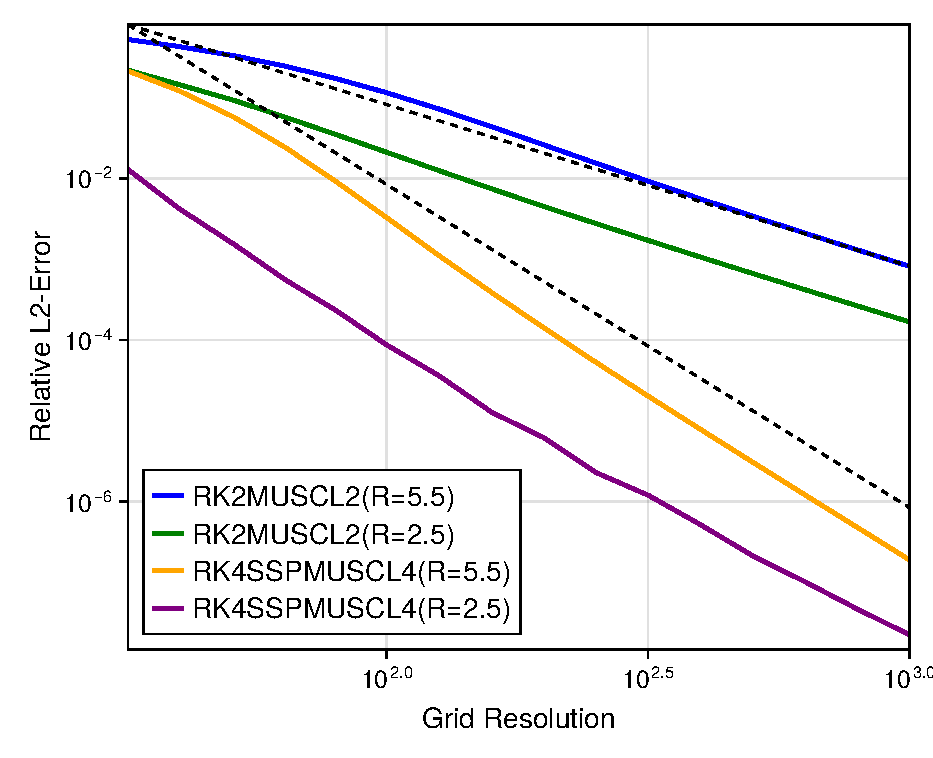
\includegraphics[width=\textwidth]{figures/advection_conv_radius.pdf}
\caption{linear advection, $t=1$}
\end{subfigure}\hfill
\begin{subfigure}{0.48\textwidth}\centering
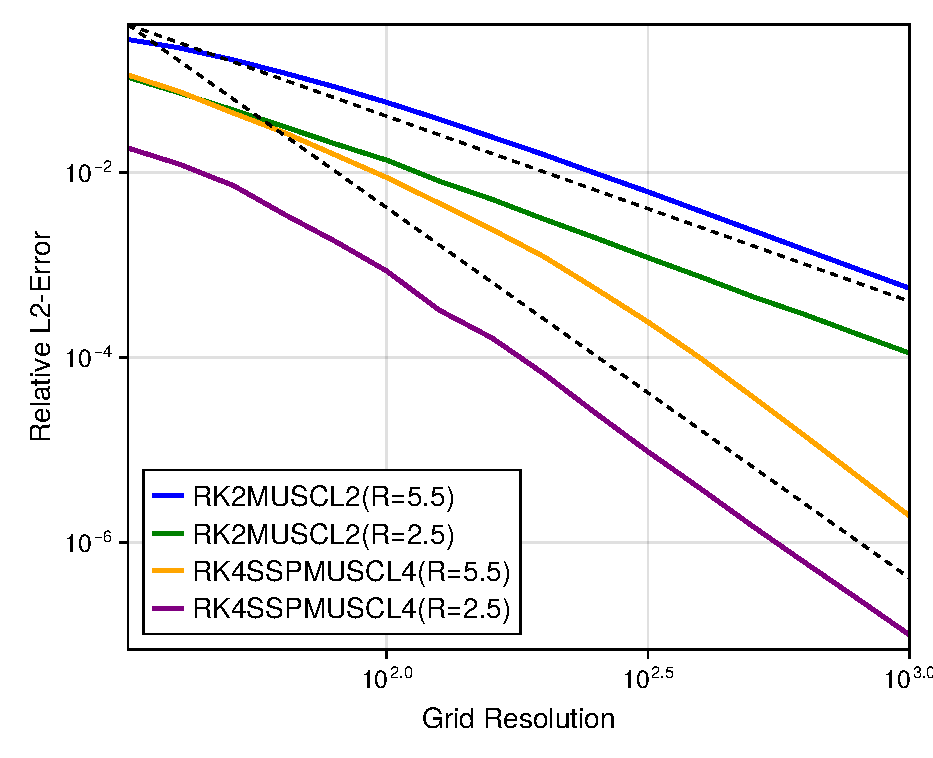
\includegraphics[width=\textwidth]{figures/burgers_conv_radius.pdf}
\caption{Burgers equation, $t=0.5$}
\end{subfigure}
\caption{Relative discrete $L^2$ errors $\big(\sum_i|U_i-u(x_i,t)|^2\big)^{1/2}/\big(\sum_iu(x_i,t)^2\big)^{1/2}$ for the Gaussian pulse in two dimensions on $N\times N$ particles in $[-5,5]^2$ perturbed by $0.2h$ (``grid resolution'' $N$, $h=10/N$), without limiter or MOOD, for RK2MUSCL2 and RK4SSPMUSCL4 with the support radii $R=2.5h$ and $R=5.5h$; dashed lines: slopes $-2$ and $-4$}\label{fig:convergence}
\end{figure}

The smaller radius $\kappa=2.5$ of the shock computations keeps the design orders on lattices (in two dimensions $2.02$, $3.00$, $4.01$ for advection and $2.06$, $2.98$, $4.12$ for Burgers) with errors at the finest resolution that are $5$ to $30$ times smaller than with $\kappa=5.5$ in two dimensions ($42$ times for $K=4$ in one dimension), since the fits weight the near neighbours more strongly; the exception is $K=3$ in one dimension, which falls back to the derivative degree two (\cref{sec:recfit}) and is of second order. \Cref{fig:convergence} shows that on the perturbed clouds the radius acts mainly on the error constant. For $K=2$ the curves of both radii are parallel, and at $N=1000$ the relative $L^2$ errors with $\kappa=2.5$ are $4.9$ (advection) and $5.0$ (Burgers) times smaller than with $\kappa=5.5$. For $K=4$ the factors are $8.5$ and $19$. $K=2$ and $K=3$ keep their orders on the perturbed clouds ($1.97$--$2.00$ and $2.91$ in two dimensions, \cref{tab:convergence}), whereas $K=4$ with $\kappa=2.5$ drops to $2.98$ in one dimension, $3.24$ for two-dimensional advection and $3.78$ for Burgers, visible in \cref{fig:convergence} as the less regular slope of the curve RK4SSPMUSCL4($R=2.5$): with $0.2h$ perturbations some stencils of radius $2.5h$ are too close to the minimal size for the degree-three fits. In two dimensions the errors of $K=4$ with $\kappa=2.5$ are nevertheless smaller than with $\kappa=5.5$ over the whole range tested ($1.1\cdot10^{-7}$ instead of $1.4\cdot10^{-6}$ in $L^1$ for Burgers at $N=1000$); in one dimension they are about $20\%$ larger at $N=3163$. For the full order of $K=4$ on perturbed clouds, $\kappa$ between $3.5$ and $5.5$ is needed.

\subsection{Mass conservation}\label{sec:mass}

Summing the volume-weighted updates \eqref{eq:scheme} over all interior particles shows that the scheme is conservative if the generalized face vectors $S_{ij}=2V_ic_{ij}$ are antisymmetric, $S_{ij}=-S_{ji}$, like the normals of a mesh face seen from its two cells. The MLS weights have this property on lattices with equal volumes, but not on irregular clouds: on the perturbed lattices of our experiments the relative pair defects $|V_ic_{ij}+V_jc_{ji}|$ are about $6\%$ for degree one and $17\%$ for degree three, and $73\%$ for pairs whose two particles use different derivative degrees, which the coupled mode creates at the boundaries of every lowered region. Meshless coefficients that are exactly antisymmetric can be constructed \cite{Chiu2011,Chiu2012,Suchde2017}; we do not apply such a correction here. To measure the effect, we report the \emph{conservation defect}
\begin{equation}\label{eq:defect}
\delta_m = \frac{m(t_{\mathrm{end}})-m(0)-\Phi(t_{\mathrm{end}})}{m(t_{\mathrm{end}})},
\end{equation}
with the discrete mass $m(t)=\bar h^D\sum_{i\in I}U_i$, the equal volumes $\bar h^D=|\Omega|/|I|$ and the exact time-integrated boundary flux $\Phi$, for a one-dimensional Burgers shock: $u=1$ for $x<-2$ and $u=0$ for $x>-2$ on $[-5,5]$ with transmissive boundaries, up to $t=10$, so $\Phi=\tfrac12t$. We use $N=32,\dots,3163$ particles perturbed by $0.4h$, $\kappa=5.5$, $\CFL=0.2$ and the aligned flux. The full study, including smooth and two-dimensional problems, other perturbations and radii, the limiters and the geometric flux, is part of the supplementary material.

\begin{figure}[!htbp]
\centering
\begin{subfigure}{0.48\textwidth}\centering
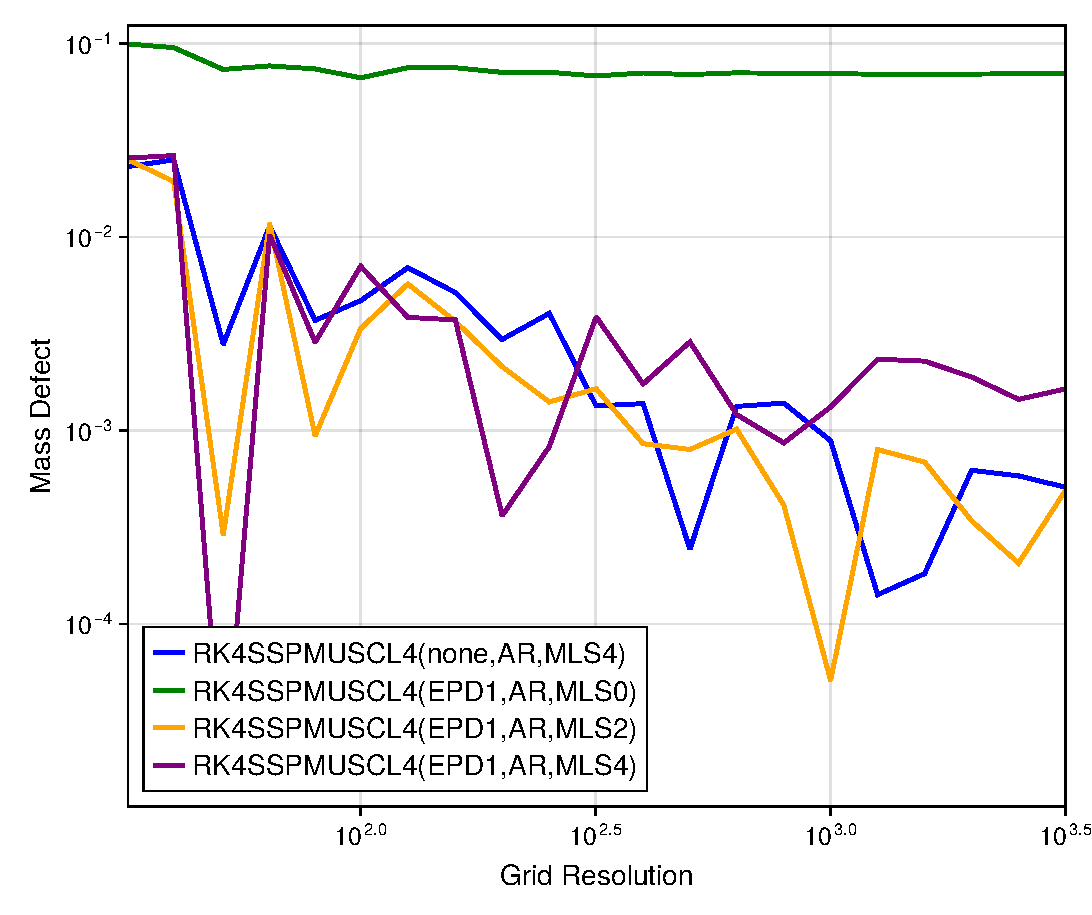
\includegraphics[width=\textwidth]{figures/shock_mass_defect_epd1.pdf}
\caption{MOOD with EPD1}
\end{subfigure}\hfill
\begin{subfigure}{0.48\textwidth}\centering
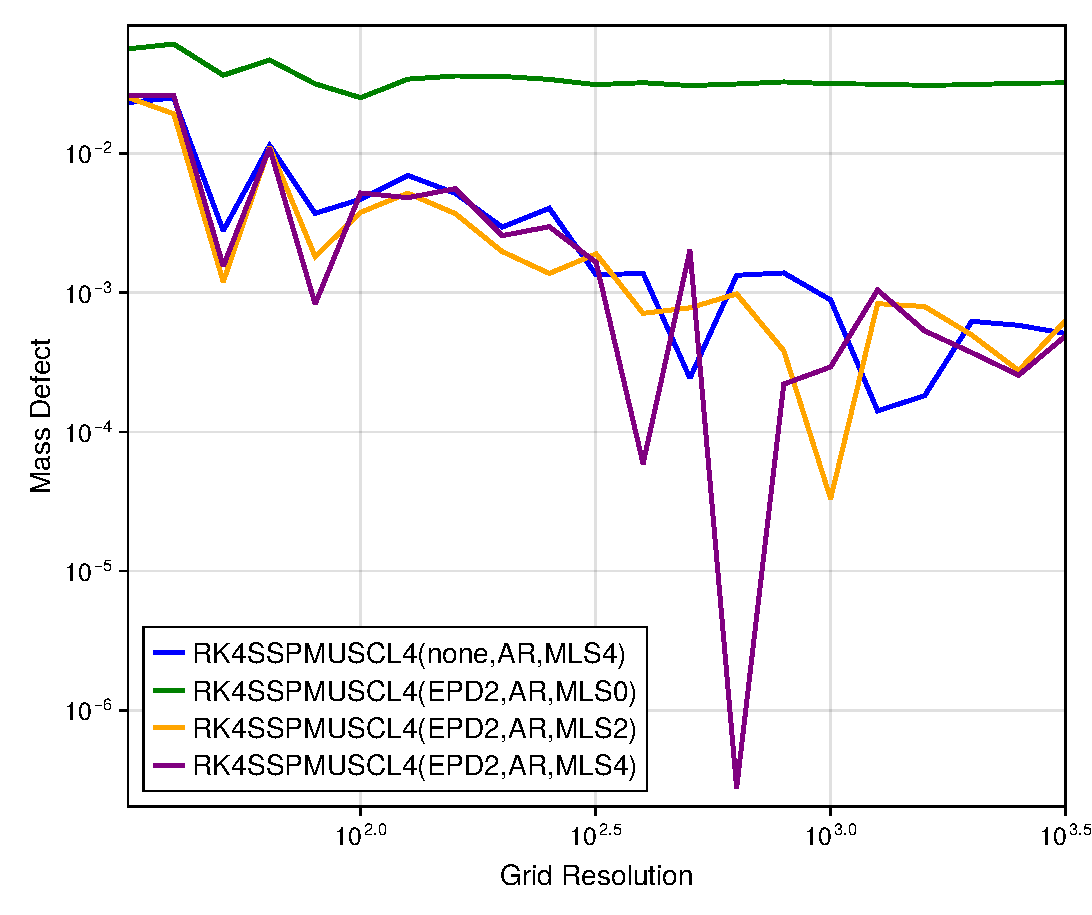
\includegraphics[width=\textwidth]{figures/shock_mass_defect_epd2.pdf}
\caption{MOOD with EPD2}
\end{subfigure}
\caption{Conservation defect $|\delta_m|$ of \eqref{eq:defect} for the one-dimensional Burgers shock, perturbation $0.4h$, $\kappa=5.5$, aligned flux, for RK4SSPMUSCL4 without MOOD (MLS4) and with MOOD in the coupled mode (MLS0) and in the frozen mode with $k_{\mathrm{div}}=2$ (MLS2) and $k_{\mathrm{div}}=4$ (MLS4)}\label{fig:mass}
\end{figure}

\Cref{fig:mass} shows the main effects. Without MOOD and in the frozen mode with $k_{\mathrm{div}}=2$, the defect decreases under refinement, at rates between $0.7$ and $1$, to a few $10^{-4}$ at $N=3163$, which is the resolution of this test: even on the unperturbed lattice, the position of the inflow boundary and of the initial jump causes defects of up to half a particle of the inflow state. The coupled mode changes the mass by several percent ($3$--$14\%$ for $K=3,4,5$), and this defect does not decrease under refinement; the coupled mode should therefore not be used for $K\ge3$. The frozen mode with $k_{\mathrm{div}}=K$ avoids mixed degrees; its defects mostly decrease like those of the unstabilized scheme, except for EPD1 with $K=4$, whose defect stays at about $10^{-3}$ in the range tested, and for $K=5$, where some stencils are too small for the degree-five fit and fall back to a lower degree. The difference between mixed and equal degrees has a simple explanation: the pairs of a high-degree and a low-degree particle at the boundary of a lowered region have the same arrangement wherever the shock is, so their defects have a systematic sign and accumulate, whereas with equal degrees on a randomly perturbed cloud the defects of the pairs at the shock change sign as the shock moves and largely cancel. For smooth solutions the defects caused by the irregular cloud are small, about $10^{-4}$ in two dimensions at $N=200$, and decrease under refinement.

\subsection{The Sod shock tube}\label{sec:sod}

As a one-dimensional test for systems we use the shock tube of Sod \cite{Sod1978}: $(\rho,u,p)=(1,0,1)$ for $x<0$ and $(0.125,0,0.1)$ for $x>0$ on $[-0.5,0.5]$, $\gamma=1.4$, up to $t=0.2$, with a Dirichlet condition on the left and a transmissive condition on the right. The clouds are lattices perturbed by $0.2h$ with $N=100,\dots,1000$ particles (eleven resolutions), $\kappa=5.5$, $\alpha=1$ and $\CFL=0.2$. We compare RK2MUSCL1, RK2MUSCL2 with EPD1, EPD2 and the VK limiter, and RK3MUSCL3 and RK4SSPMUSCL4 with EPD1 and EPD2 in the frozen mode with $k_{\mathrm{div}}=2$ and $k_{\mathrm{div}}=K$, all with the aligned flux except RK2MUSCL1. The errors are measured against the exact Riemann solution. \Cref{fig:sod} shows the profiles at $N=200$ and \cref{tab:sod} the errors.

\begin{figure}[!htbp]
\centering
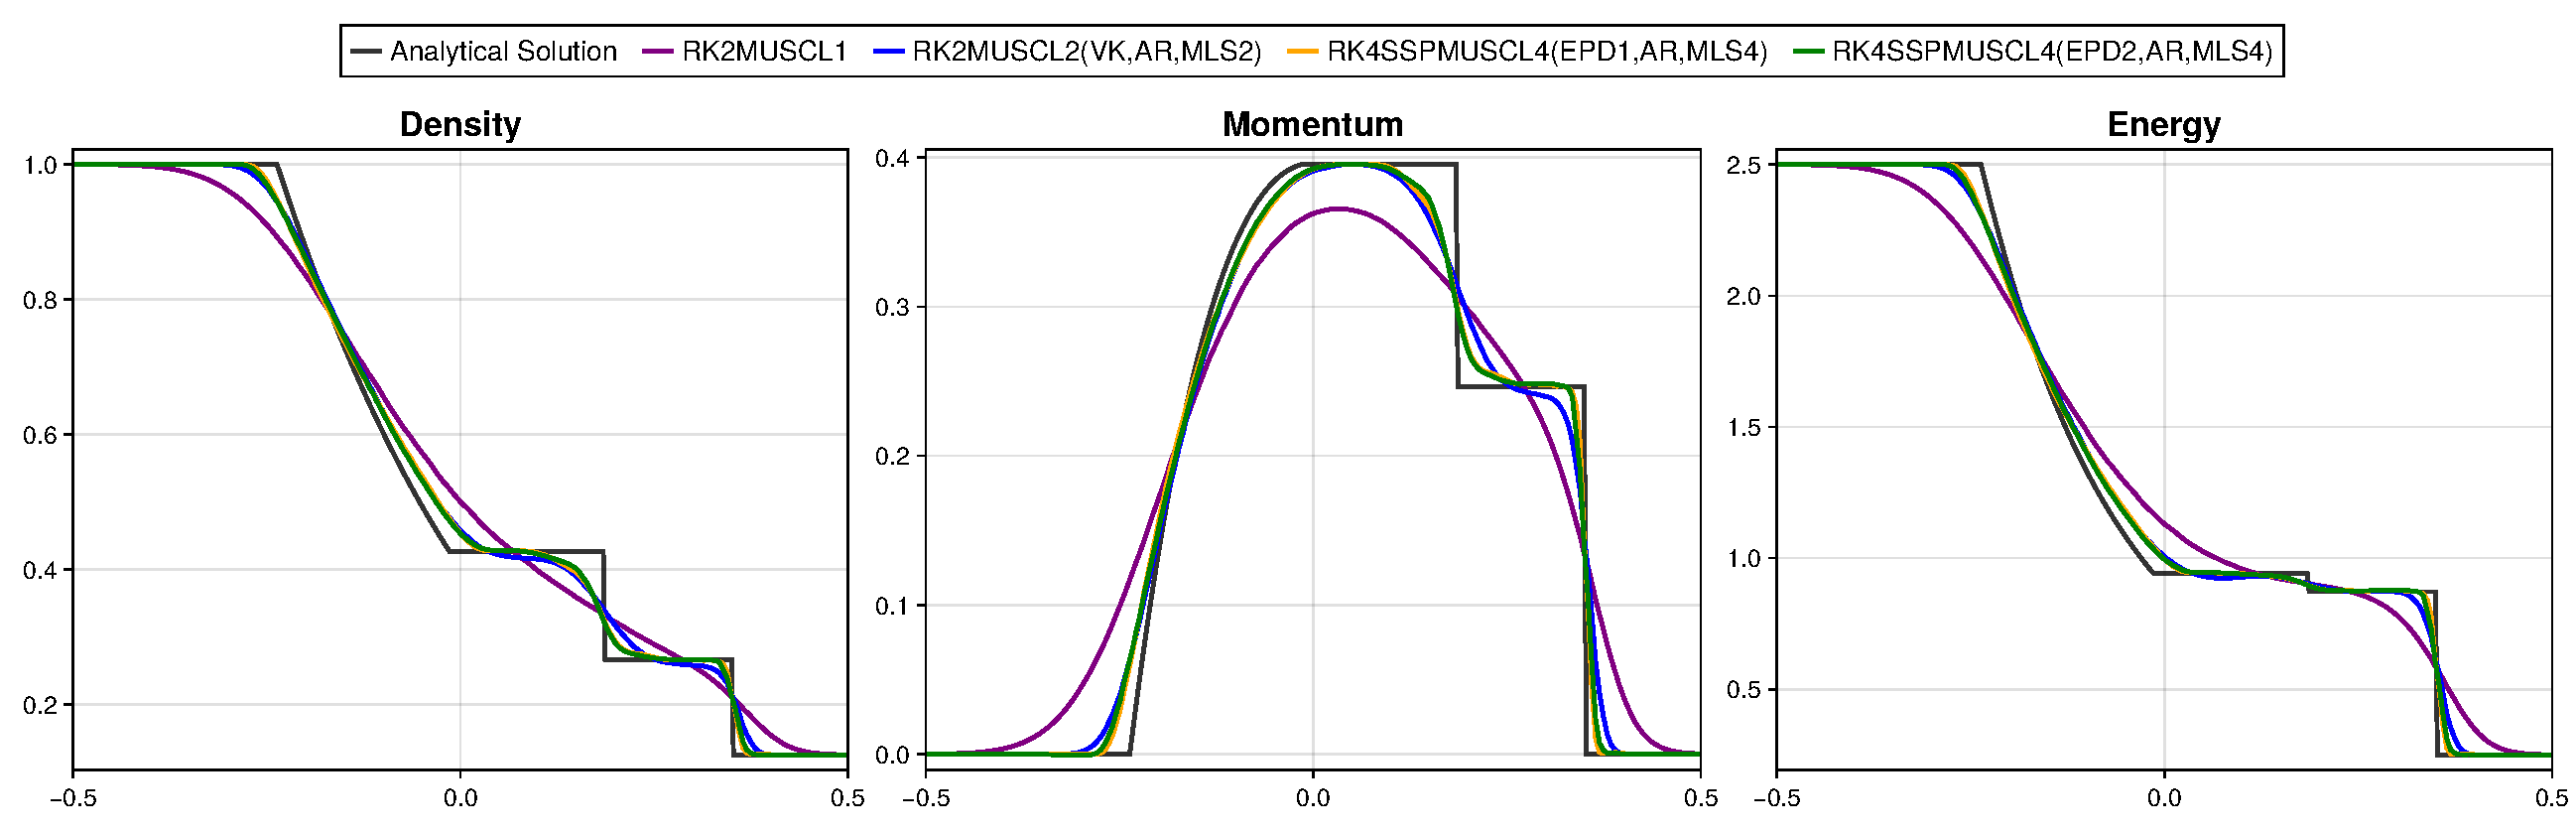
\includegraphics[width=\textwidth]{figures/euler_sod_components.pdf}
\caption{Sod shock tube at $t=0.2$ on $N=200$ particles perturbed by $0.2h$, $\kappa=5.5$: density, momentum and energy of RK2MUSCL1, RK2MUSCL2(VK,MLS2), RK4SSPMUSCL4(EPD1,MLS4) and RK4SSPMUSCL4(EPD2,MLS4), and the exact solution; all schemes except RK2MUSCL1 use the aligned flux}\label{fig:sod}
\end{figure}

\begin{table}[!htbp]
\centering
\caption{Sod shock tube at $t=0.2$, perturbation $0.2h$, $\kappa=5.5$: discrete $L^1$ and $L^2$ errors of the density against the exact solution, observed orders between $N=502$ and $N=1000$, and the relative mass change $m(t)/m(0)-1$ at $N=1000$.}\label{tab:sod}
\footnotesize
\setlength{\tabcolsep}{4pt}
\begin{adjustbox}{max width=\textwidth}
\begin{tabular}{lccccccc}
\toprule
& \multicolumn{4}{c}{$L^1(\rho)$} & \multicolumn{2}{c}{$L^2(\rho)$} & \\
\cmidrule(lr){2-5}\cmidrule(lr){6-7}
& $N=100$ & $N=317$ & $N=1000$ & order & $N=1000$ & order & mass, $N=1000$\\
\midrule
RK2MUSCL1 & 4.51e-2 & 2.91e-2 & 1.55e-2 & 0.59 & 2.49e-2 & 0.42 & $+$2.5e-5\\
RK2MUSCL2(EPD1,MLS2) & 2.63e-2 & 1.32e-2 & 4.68e-3 & 0.87 & 1.17e-2 & 0.55 & $+$3.3e-5\\
RK2MUSCL2(EPD2,MLS2) & 3.06e-2 & 1.52e-2 & 5.49e-3 & 0.92 & 1.28e-2 & 0.57 & $+$3.2e-5\\
RK2MUSCL2(VK,MLS2) & 2.97e-2 & 1.05e-2 & 3.57e-3 & 0.97 & 1.01e-2 & 0.52 & $+$3.1e-5\\
RK3MUSCL3(EPD1,MLS2) & 2.89e-2 & 1.00e-2 & 3.30e-3 & 1.00 & 1.02e-2 & 0.54 & $+$3.3e-5\\
RK3MUSCL3(EPD2,MLS2) & 2.97e-2 & 1.49e-2 & 5.25e-3 & 0.92 & 1.26e-2 & 0.57 & $+$3.3e-5\\
RK3MUSCL3(EPD1,MLS3) & 2.81e-2 & 9.64e-3 & 3.16e-3 & 1.00 & 9.62e-3 & 0.57 & $+$6.0e-5\\
RK3MUSCL3(EPD2,MLS3) & 2.84e-2 & 9.48e-3 & 3.12e-3 & 1.02 & 9.49e-3 & 0.57 & $+$1.2e-4\\
RK4SSPMUSCL4(EPD1,MLS2) & 2.58e-2 & 8.67e-3 & 2.80e-3 & 1.00 & 9.61e-3 & 0.51 & $+$3.2e-5\\
RK4SSPMUSCL4(EPD2,MLS2) & 2.88e-2 & 1.41e-2 & 4.93e-3 & 0.93 & 1.18e-2 & 0.58 & $+$3.6e-5\\
RK4SSPMUSCL4(EPD1,MLS4) & 2.56e-2 & 8.18e-3 & 2.65e-3 & 1.05 & 8.24e-3 & 0.61 & $+$8.0e-5\\
RK4SSPMUSCL4(EPD2,MLS4) & 2.59e-2 & 8.27e-3 & 2.72e-3 & 1.06 & 8.39e-3 & 0.61 & $+$1.0e-4\\
\bottomrule
\end{tabular}
\end{adjustbox}
\end{table}

All 132 runs reach the final time with positive density and pressure; the minimum density is that of the exact right state, $0.125$, in all runs except RK2MUSCL2(EPD1), where it is $0.1249$. For every scheme with $K\ge2$ the $L^1$ error decreases with orders between $0.87$ and $1.06$, the rate expected for a solution with a shock, and the $L^2$ error with orders between $0.51$ and $0.61$; RK2MUSCL1 is not yet in its asymptotic range ($0.59$). The frozen mode with $k_{\mathrm{div}}=K$ gives the smallest errors, $3.1\cdot10^{-3}$ for $K=3$ and $2.7\cdot10^{-3}$ for $K=4$ at $N=1000$, $5.0$ and $5.8$ times less than RK2MUSCL1. With $k_{\mathrm{div}}=2$, EPD2 gains little over the second-order scheme ($5.2\cdot10^{-3}$ and $4.9\cdot10^{-3}$ for $K=3,4$, compared with $5.5\cdot10^{-3}$ for $K=2$), EPD1 more ($3.3\cdot10^{-3}$ and $2.8\cdot10^{-3}$, compared with $4.7\cdot10^{-3}$). At $K=2$ the VK limiter ($3.6\cdot10^{-3}$) is more accurate than both MOOD variants. In \cref{fig:sod} the fourth-order schemes resolve the contact discontinuity and the shock over a few particles, with at most small overshoots, while RK2MUSCL1 smears all three waves; RK2MUSCL2(VK) lies in between, with a visibly wider contact and shock. Since the waves stay inside the domain and $u=0$ in both boundary states, the exact mass is constant. Near both boundaries the state stays constant, so that the zero row sums make the updates there vanish and the boundaries cannot change the mass. The measured mass changes of $2.5\cdot10^{-5}$ to $1.2\cdot10^{-4}$ at $N=1000$ are therefore the static asymmetry of the derivative weights at the moving shock and contact; they are largest with $k_{\mathrm{div}}=K$, whose degree-three weights have the larger pair defects (\cref{sec:mass}).

\subsection{Two-dimensional shock problems}\label{sec:euler2d}

The two-dimensional Riemann problem and the double Mach reflection were computed with the first-order baseline RK2MUSCL1 (plain Rusanov flux) and, with the aligned flux, MUSCL2 with EPD1, EPD2 and the VK limiter, and MUSCL3 and MUSCL4 with EPD1 and EPD2 in the frozen mode with $k_{\mathrm{div}}=2$ and $k_{\mathrm{div}}=K$ and in the coupled mode, and MUSCL2 to MUSCL4 with EPD2 and $k_{\mathrm{div}}=2$ also with the geometric flux; the coupled MUSCL4 runs of the double Mach reflection use $960\times300$ particles. \Cref{tab:euler2d} summarizes positivity and mass. All 38 runs, and three Riemann runs with transmissive boundaries (\cref{sec:riemann}), reach the final time with positive density and pressure and without invalid values, including the coupled mode. On the Riemann problem, the minimum pressures of the second- to fourth-order schemes, $0.018$ to $0.029$, undershoot the lowest initial pressure $0.029$ by up to $39\%$; the lowest values occur with EPD1 and $k_{\mathrm{div}}=K$. With $k_{\mathrm{div}}=2$ the aligned and the geometric flux agree to within about $4\%$ in all quantities of \cref{tab:euler2d}, and the high-order schemes take as many time steps as the second-order scheme; with $k_{\mathrm{div}}=K$ and in the coupled mode they take about three times as many (\cref{sec:timestep}).

In the frozen mode the final masses agree with that of RK2MUSCL2(EPD1) to within $0.25\%$ on both problems. Since the problems have inflow and outflow boundaries, the reference is a computed mass, and the masses are known to three digits, i.e.\ to about $0.1\%$. The coupled mode with EPD1 is not conservative: its final mass differs by $+5.4\%$ ($K=3$) and $+4.7\%$ ($K=4$) on the double Mach reflection and by $+1.4\%$ ($K=3$) on the Riemann problem, consistent with \cref{sec:mass}; with EPD2 the differences are smaller, $-0.3$ to $+0.7\%$.

\begin{table}[!htbp]
\centering
\caption{Two-dimensional shock problems: minimum particle pressure and final mass relative to RK2MUSCL2(EPD1,AR,MLS2) (total masses known to about $0.1\%$). Pairs of values: EPD1 / EPD2. All runs except RK2MUSCL1 with the aligned flux. $^*$: $960\times300$ particles; the mass is still compared with the $1440\times450$ run of RK2MUSCL2(EPD1).}\label{tab:euler2d}
\scriptsize
\setlength{\tabcolsep}{2.5pt}
\begin{adjustbox}{max width=\textwidth}
\begin{tabular}{@{}lcccc@{}}
\toprule
& \multicolumn{2}{c}{double Mach reflection} & \multicolumn{2}{c}{2-D Riemann problem}\\
\cmidrule(lr){2-3}\cmidrule(lr){4-5}
& $\min p$ & mass (\%) & $\min p$ & mass (\%)\\
\midrule
RK2MUSCL1 & 1.00 & $-0.2$ & 0.029 & $0.0$\\
\begin{tabular}[t]{@{}l@{}}MUSCL2\\ \quad EPD1 / EPD2 / VK\end{tabular} & \begin{tabular}[t]{@{}c@{}}\\ 1.00\end{tabular} & \begin{tabular}[t]{@{}c@{}}\\ $0.0$\end{tabular} & \begin{tabular}[t]{@{}c@{}}\\ 0.024\,/\,0.029\,/\,0.027\end{tabular} & \begin{tabular}[t]{@{}c@{}}\\ $0.0$\end{tabular}\\
MUSCL3, $k_{\mathrm{div}}=2$ & 1.00 & $0.0$ & 0.020 / 0.028 & $0.0$\\
MUSCL3, $k_{\mathrm{div}}=3$ & 0.96 / 0.99 & $-0.2$ / $0.0$ & 0.018 / 0.026 & $0.0$ / $+0.1$\\
MUSCL3, coupled & 0.96 / 0.99 & $+5.4$ / $+0.7$ & 0.023 / 0.026 & $+1.4$ / $-0.3$\\
MUSCL4, $k_{\mathrm{div}}=2$ & 1.00 & $0.0$ & 0.026 / 0.029 & $0.0$\\
MUSCL4, $k_{\mathrm{div}}=4$ & 0.91 / 0.97 & $-0.2$ / $0.0$ & 0.022 / 0.027 & $-0.1$ / $+0.1$\\
MUSCL4, coupled & 0.88$^*$ / 0.96$^*$ & $+4.7^*$ / $+0.2^*$ & 0.019 / 0.027 & $+0.4$ / $-0.1$\\
\bottomrule
\end{tabular}
\end{adjustbox}
\end{table}

\subsection{A two-dimensional Riemann problem}\label{sec:riemann}

Two-dimensional Riemann problems with four constant states in the quadrants of $[0,1]^2$ were classified by Zhang and Zheng \cite{ZhangZheng1990}, Schulz-Rinne \cite{SchulzRinne1993class} and Chang, Chen and Yang \cite{ChangChenYang1995,ChangChenYang2000}, computed systematically by Schulz-Rinne, Collins and Glaz \cite{SchulzRinne1993} and by Lax and Liu \cite{LaxLiu1998}, whose numbering we follow, and have become standard benchmarks for shock-capturing schemes \cite{KurganovTadmor2002}. We use Configuration~3 of \cite{LaxLiu1998,KurganovTadmor2002}, in which every pair of adjacent quadrants is connected by a single shock. With the discontinuities at $x=0.5$ and $y=0.5$, the initial states $(\rho,u,v,p)$ are
\[
\begin{array}{ll}
(0.5323,\,1.206,\,0,\,0.3) & (1.5,\,0,\,0,\,1.5)\\
(0.138,\,1.206,\,1.206,\,0.029) & (0.5323,\,0,\,1.206,\,0.3)
\end{array}
\]
in the upper left, upper right, lower left and lower right quadrants, and the solution is computed until $t=0.3$. Away from the centre the solution consists of plane shocks, whose positions follow from the Rankine--Hugoniot conditions: the shocks bounding the upper right state move with speed $-0.663$ and lie at $x=0.301$ and $y=0.301$ at $t=0.3$, and the shocks bounding the low-density lower left state move with speed $-0.422$ and lie at $x=0.373$ and $y=0.373$. The ghost particles carry these exact plane-shock states on all four sides. Near the centre the shocks interact: the two shocks bounding the low-density state are joined by a curved shock between two triple points, and along the diagonal a mushroom-shaped jet with two roll-ups forms. The problem is symmetric with respect to the diagonal $x=y$.

\begin{figure}[!htbp]
\centering
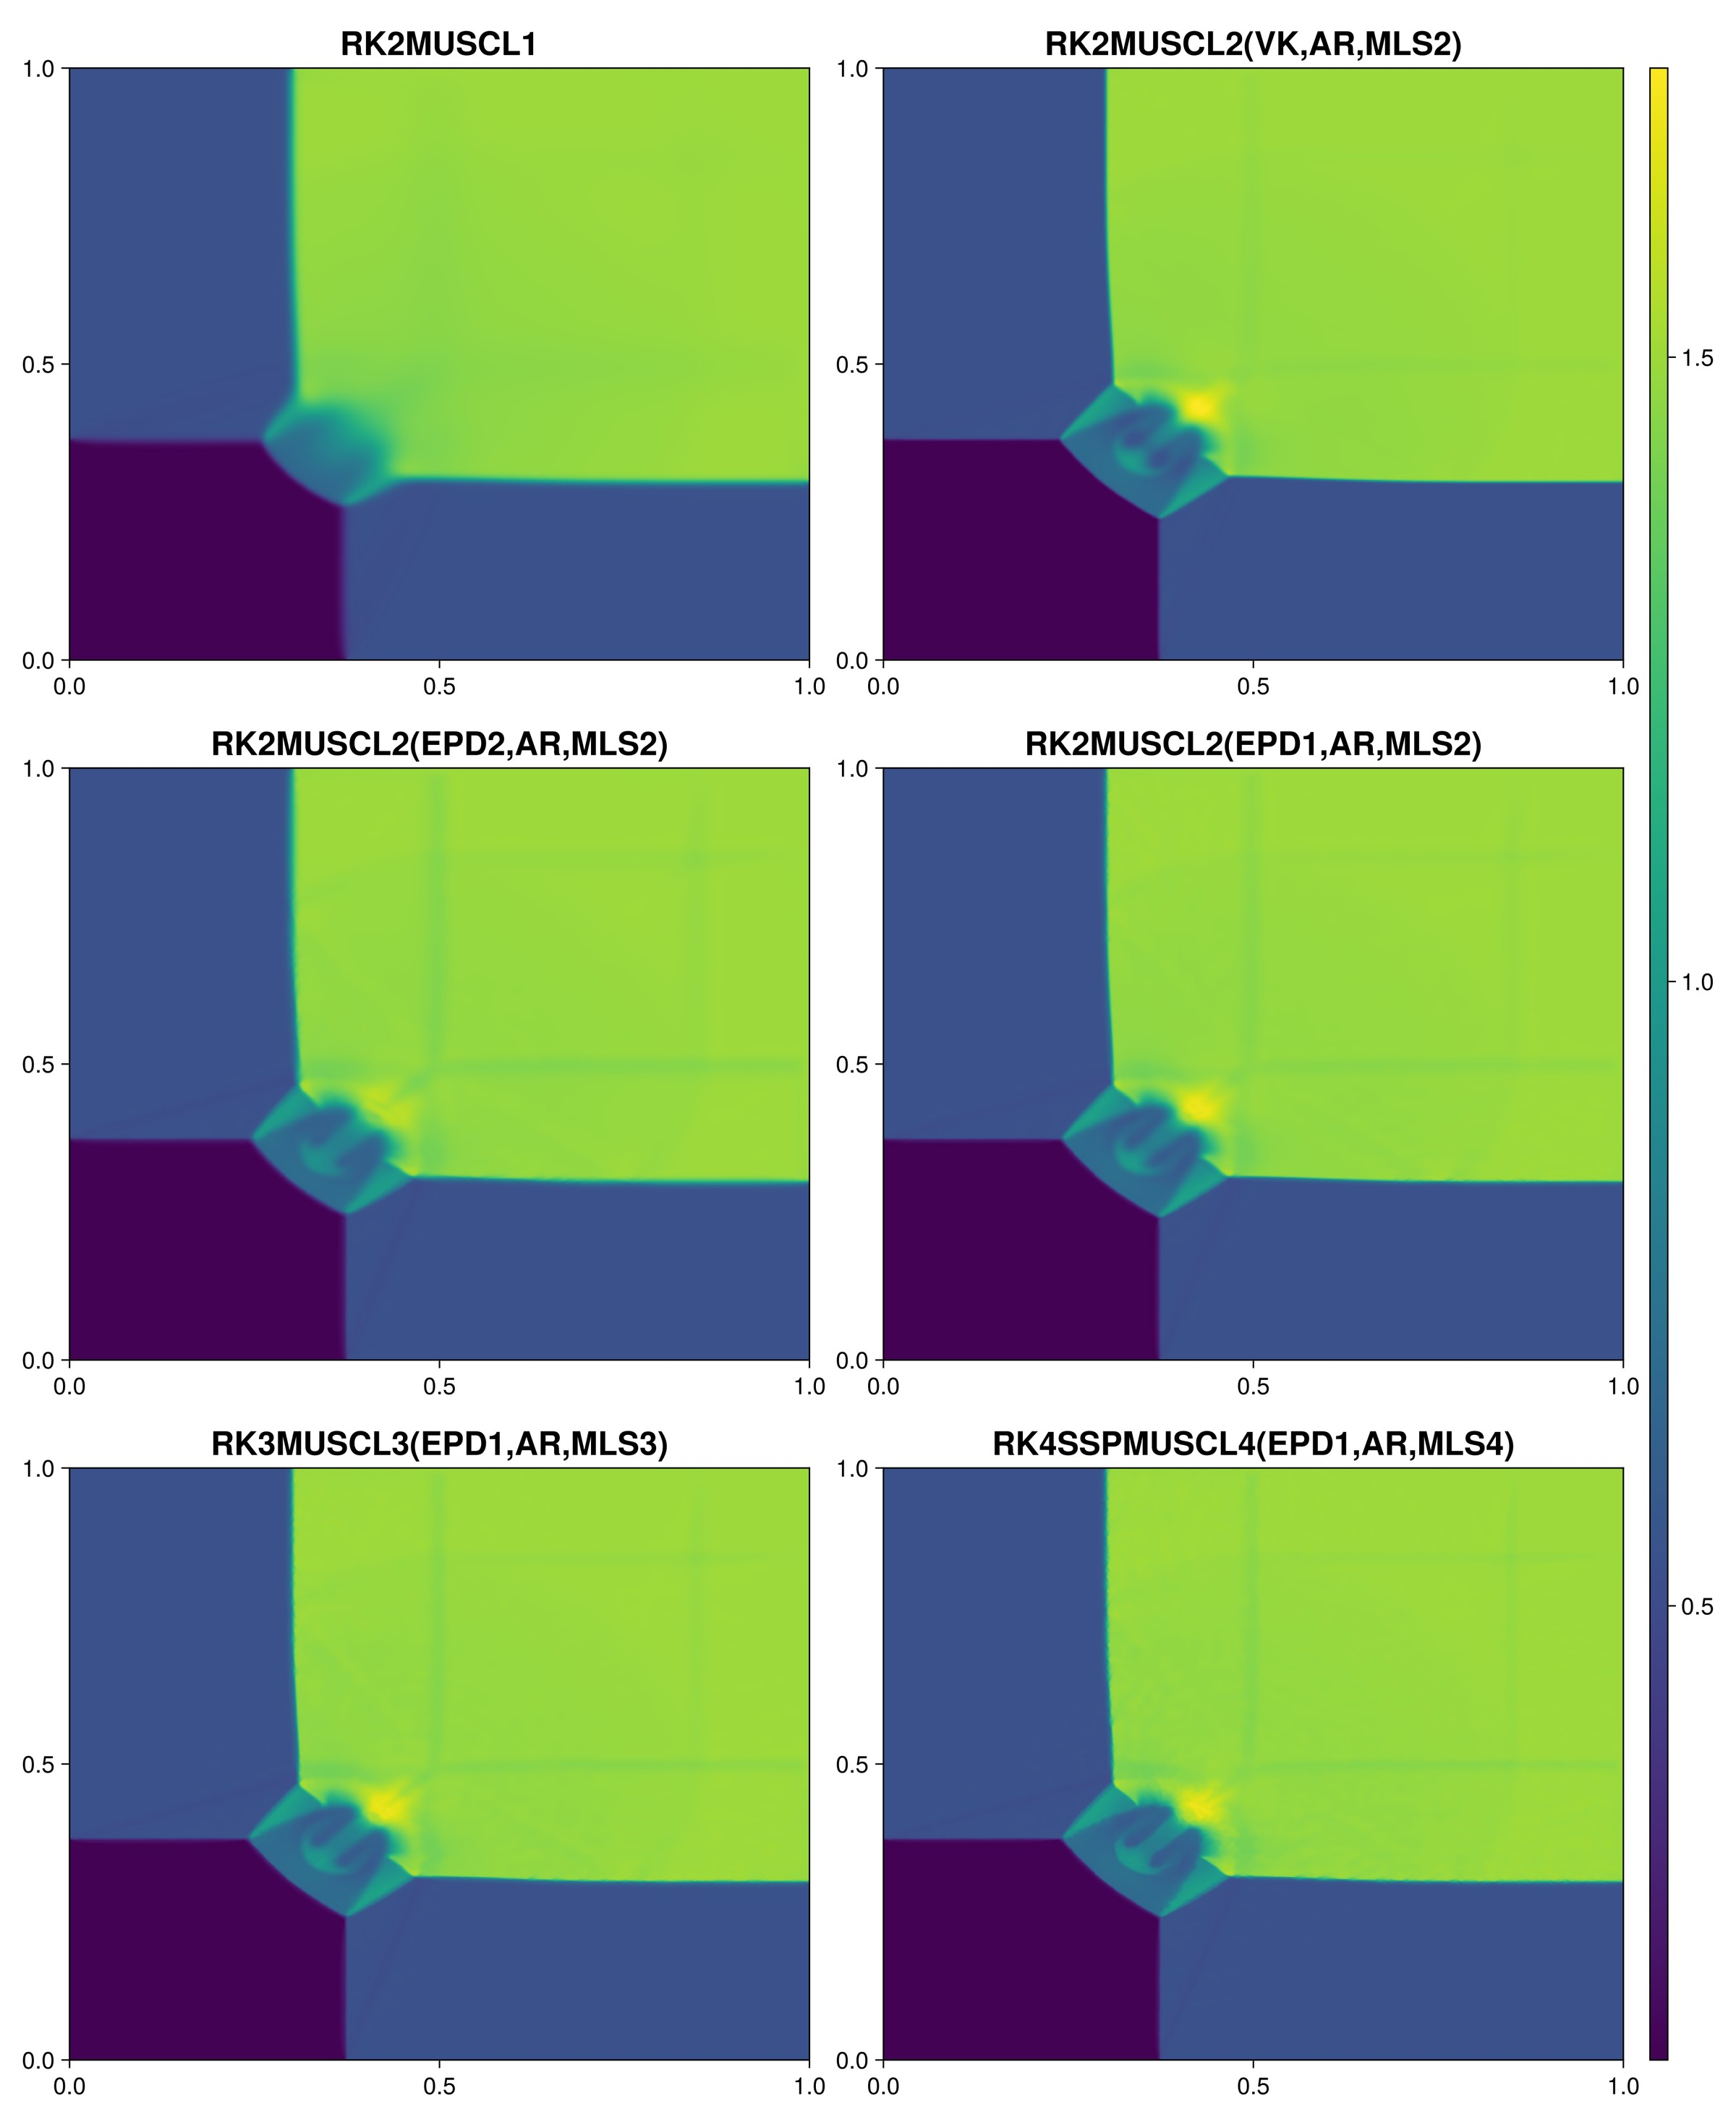
\includegraphics[width=0.74\textwidth]{figures/riemann2d_density_078.jpg}
\caption{Two-dimensional Riemann problem (Configuration~3), density at $t=0.3$ on $800\times800$ particles perturbed by $0.2h$, with a common colour scale, for RK2MUSCL1, RK2MUSCL2 with the VK limiter, EPD2 and EPD1, RK3MUSCL3(EPD1,MLS3) and RK4SSPMUSCL4(EPD1,MLS4); all schemes except RK2MUSCL1 use the aligned flux}\label{fig:riemann}
\end{figure}

\begin{figure}[!htbp]
\centering
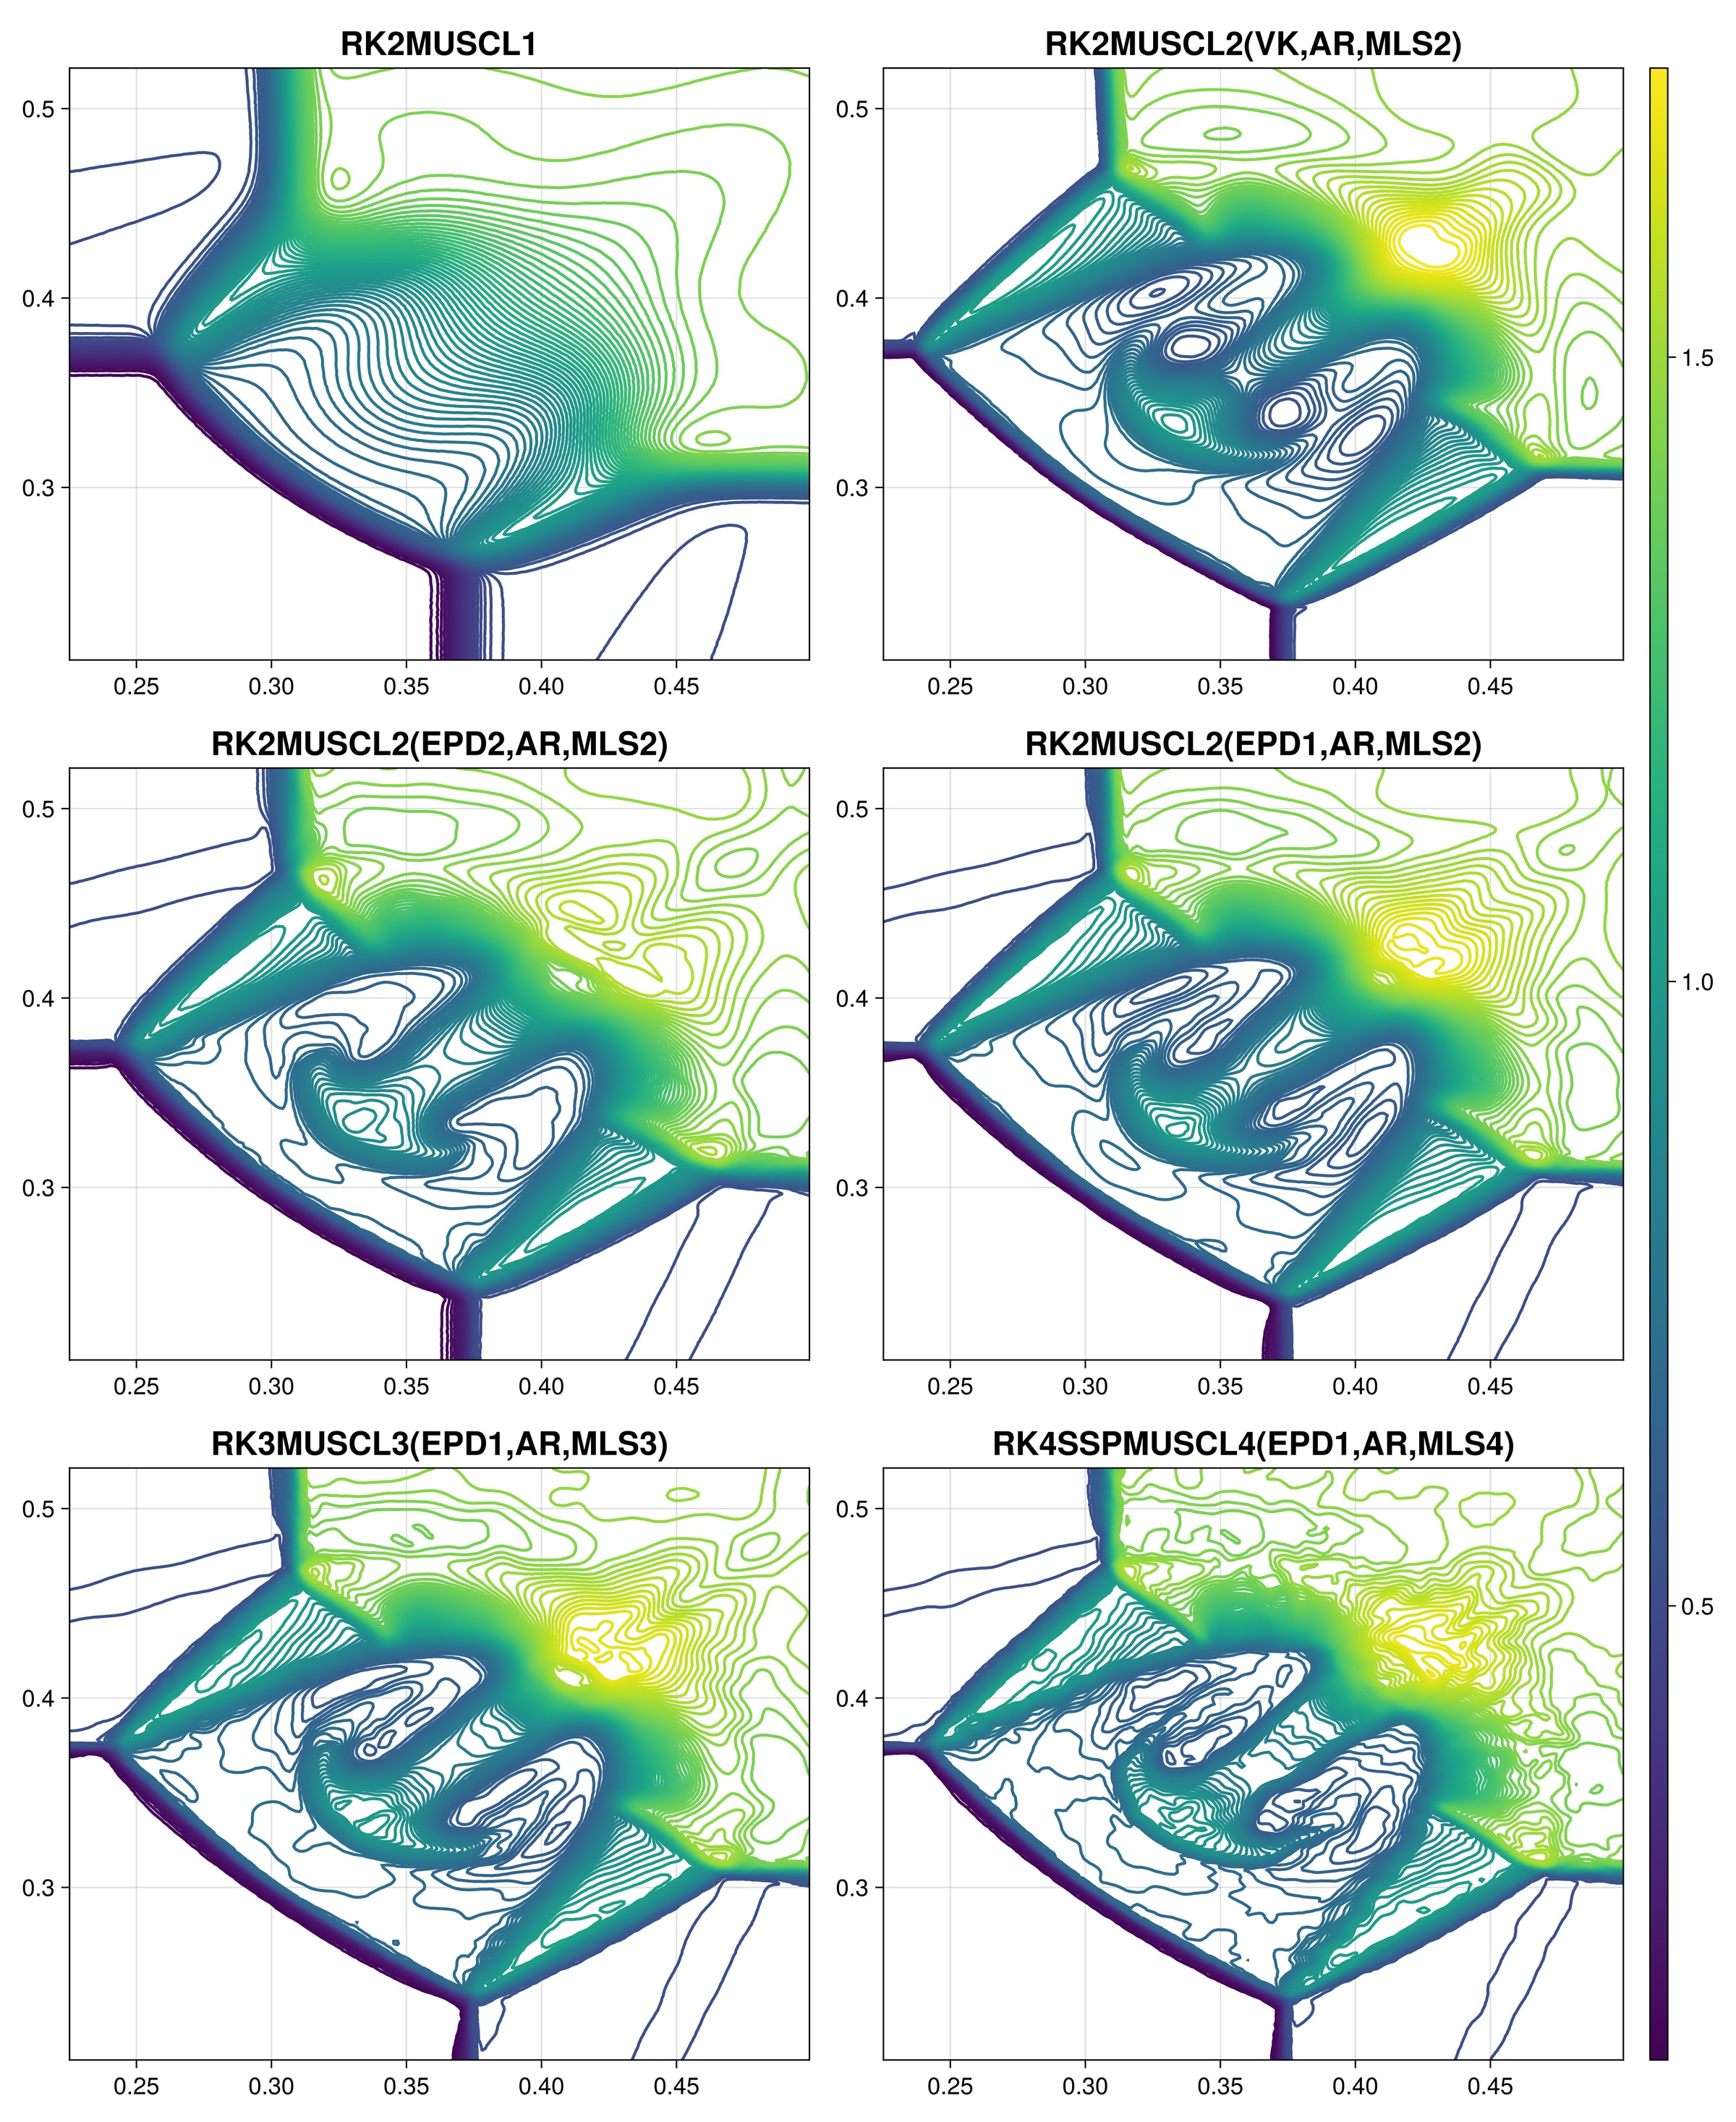
\includegraphics[width=0.74\textwidth]{figures/riemann2d_zoom_078.jpg}
\caption{Two-dimensional Riemann problem: detail $[0.225,0.5]\times[0.21,0.52]$ of \cref{fig:riemann} with $100$ contour levels}\label{fig:riemannzoom}
\end{figure}

\Cref{fig:riemann,fig:riemannzoom} show the density at $t=0.3$. All runs reproduce the expected wave pattern. With the exact boundary states, the shocks are straight up to the boundaries and lie close to their exact positions, $0.373$ and $0.301$, symmetric with respect to the diagonal. With transmissive instead of exact boundary states, the final mass of the EPD2 runs with $k_{\mathrm{div}}=2$ is $0.6\%$ ($K=2,3$) and $0.9\%$ ($K=4$) lower, a boundary effect that does not concern the interior scheme.

The resolution of the jet along the diagonal differs between the schemes. RK2MUSCL1 smears the cap of the jet into a single blob without roll-ups. The second-order runs resolve the two roll-ups of the mushroom cap; the third- and fourth-order runs resolve them with sharper gradients and a thinner stem. EPD1 and the VK limiter produce a local density maximum of about $1.7$ next to the jet, at about $(0.43,0.43)$, which EPD2 smears. In the contour lines of \cref{fig:riemannzoom} the fourth-order run shows small-scale noise in the upper right state next to the jet. The MOOD runs show faint lines along $x=0.5$ and $y=0.5$ in the upper right state of \cref{fig:riemann}, traces of the initial discontinuities in the fluid at rest, a start-up error common to shock-capturing schemes \cite{LiskaWendroff2003}. In \cref{fig:riemannzoom} faint straight contour lines run from the interaction region towards the lower right; we have not identified their origin.

\subsection{Double Mach reflection}\label{sec:dmr}

The double Mach reflection of Woodward and Colella \cite{Woodward1984} describes a Mach 10 shock that hits a $30^\circ$ wedge, so that the shock makes an angle of $60^\circ$ with the wall. In the frame of the wall, the shock initially lies on the line $x=\tfrac16+y/\sqrt3$ and separates the pre-shock state $(\rho,u,v,p)=(1.4,0,0,1)$ on the right from the post-shock state $(8,\,8.25\cos30^\circ,\,-8.25\sin30^\circ,\,116.5)$ on the left. At the bottom, the post-shock state is prescribed for $x<\tfrac16$ and a slip wall for $x\ge\tfrac16$; at the top, the ghost particles carry the exact states of the moving incident shock, $x_s(y,t)=\tfrac16+(y+20t)/\sqrt3$; the left boundary is an inflow of the post-shock state and the right boundary is transmissive. We use the reduced domain $[0,3.2]\times[0,1]$ instead of the domain $[0,4]\times[0,1]$ of Woodward and Colella; it contains all waves until $t=0.2$.

\begin{figure}[!htbp]
\centering
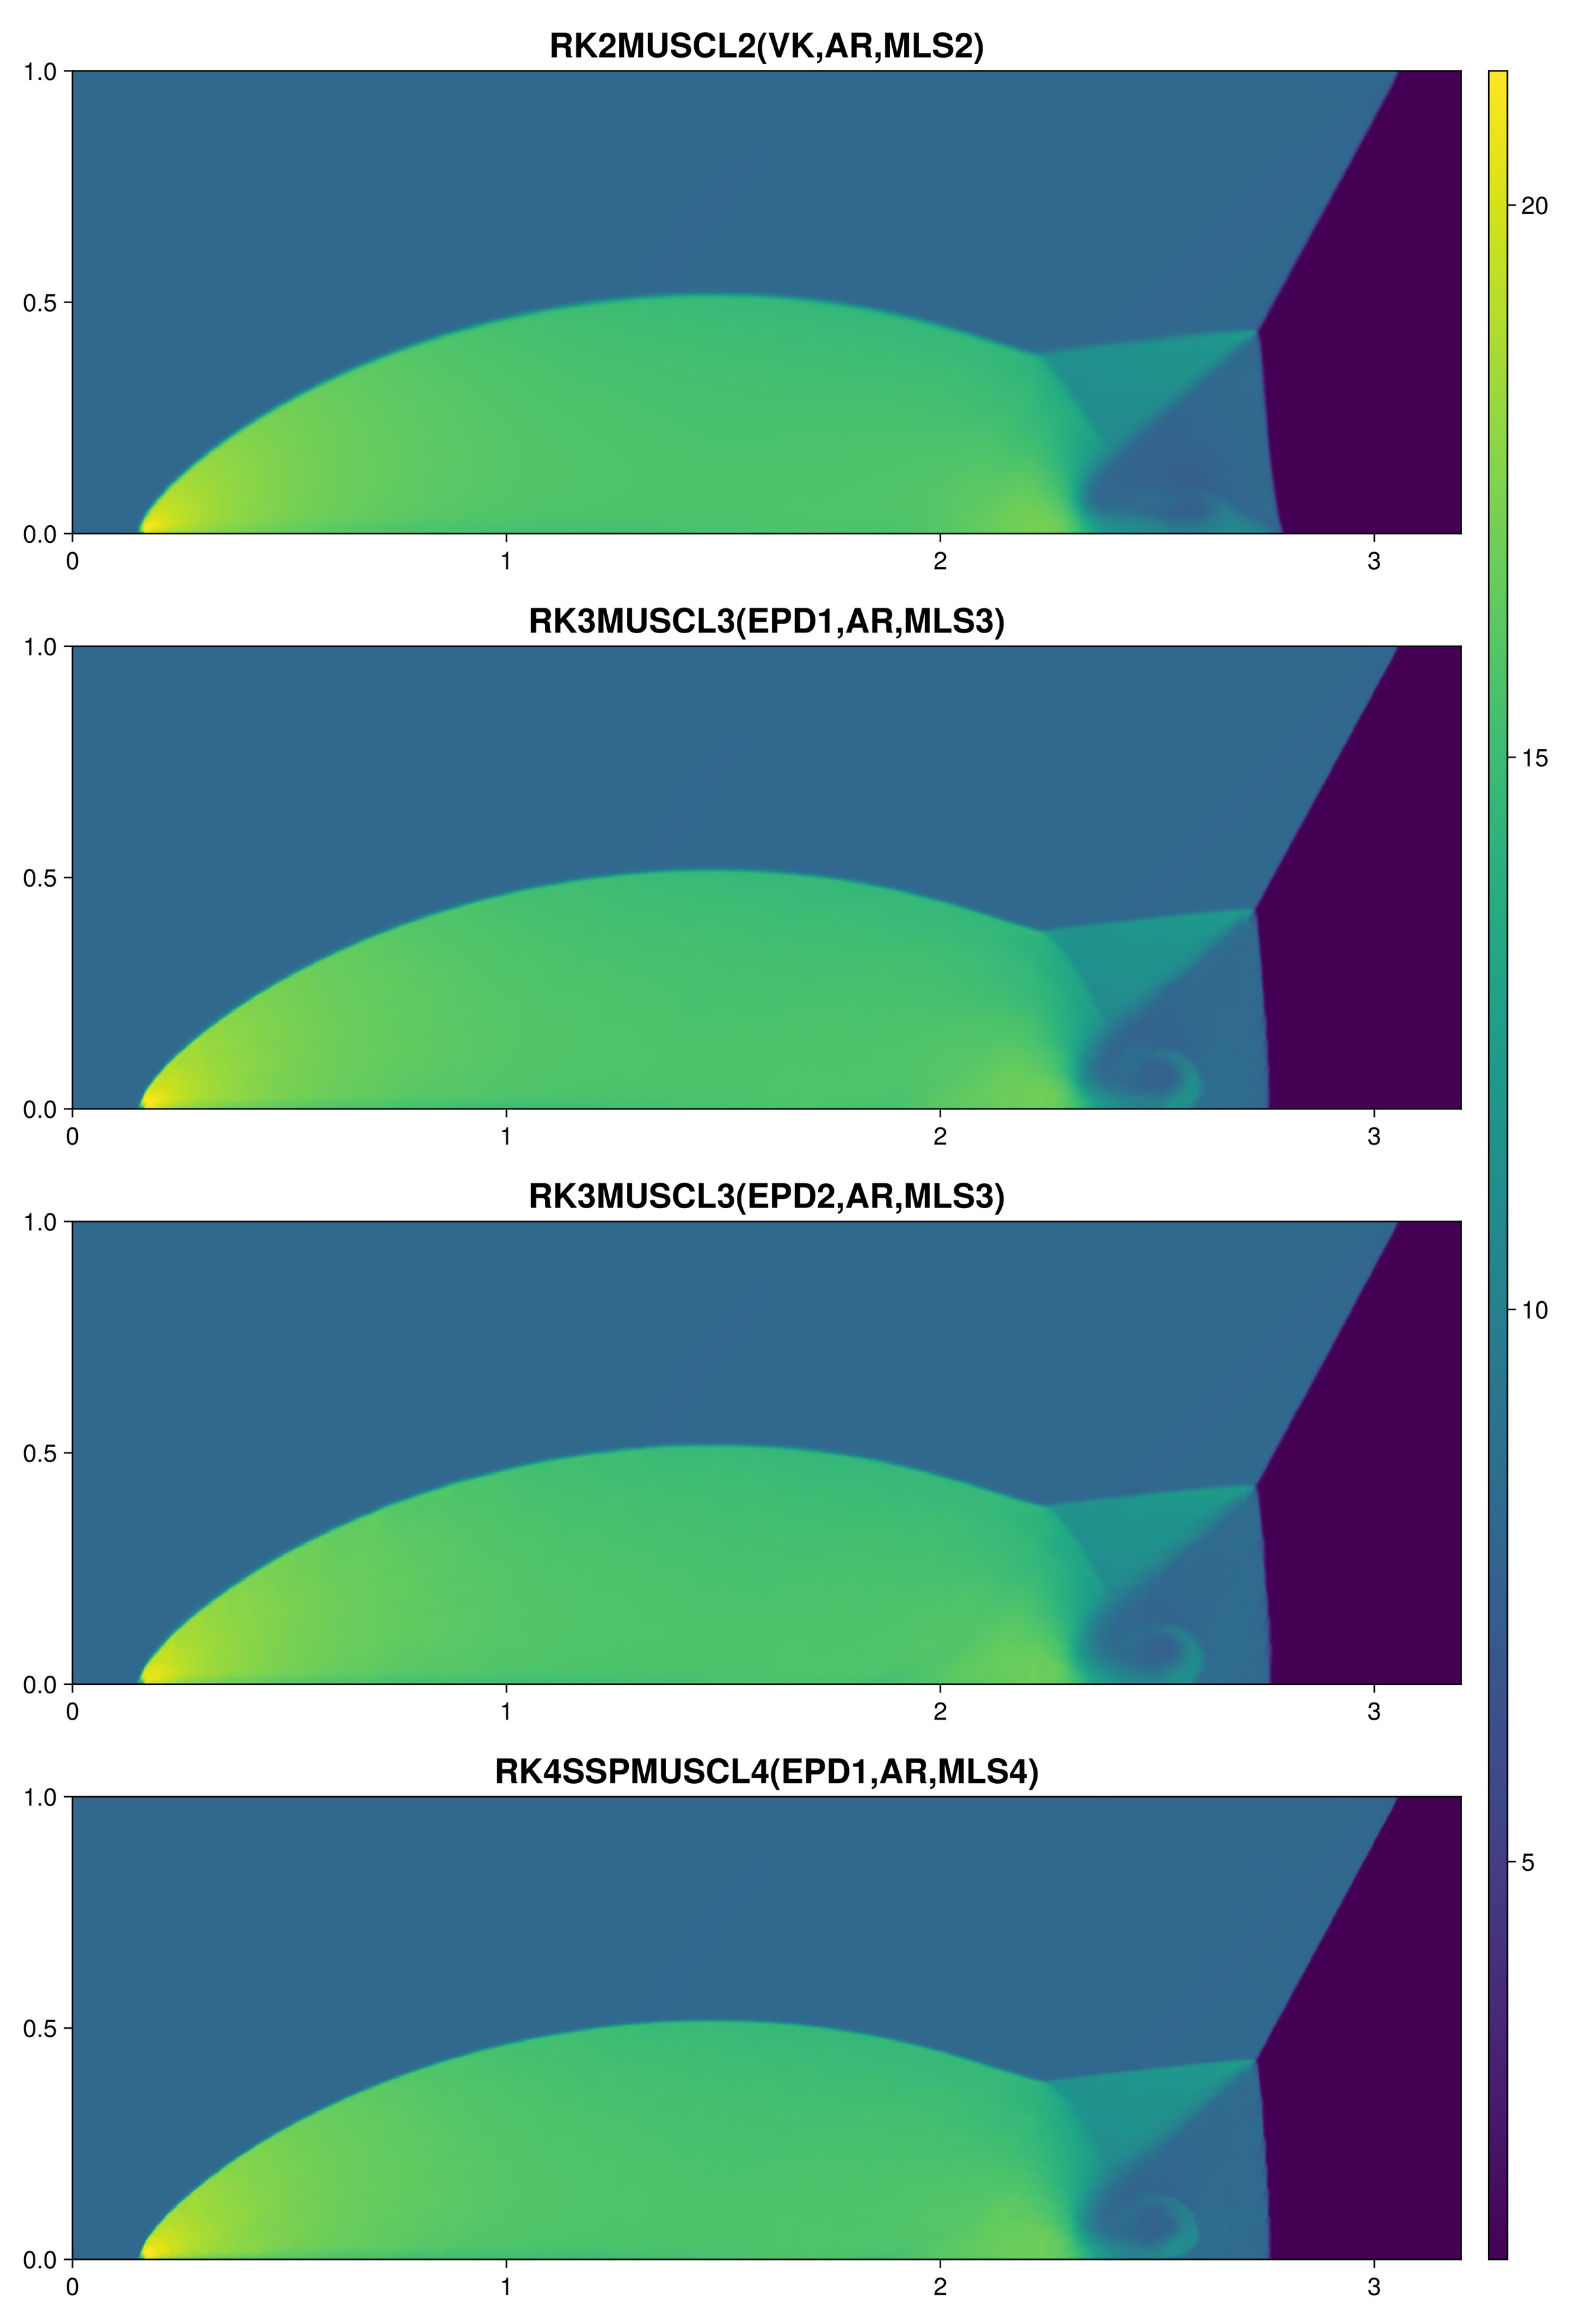
\includegraphics[width=0.72\textwidth]{figures/dmr_density_078.jpg}
\caption{Double Mach reflection, density at $t=0.2$ on $1440\times450$ particles perturbed by $0.2h$ for RK2MUSCL2(VK), RK3MUSCL3(EPD1,MLS3), RK3MUSCL3(EPD2,MLS3) and RK4SSPMUSCL4(EPD1,MLS4), all with the aligned flux, with a common colour scale}\label{fig:dmr}
\end{figure}

\begin{figure}[!htbp]
\centering
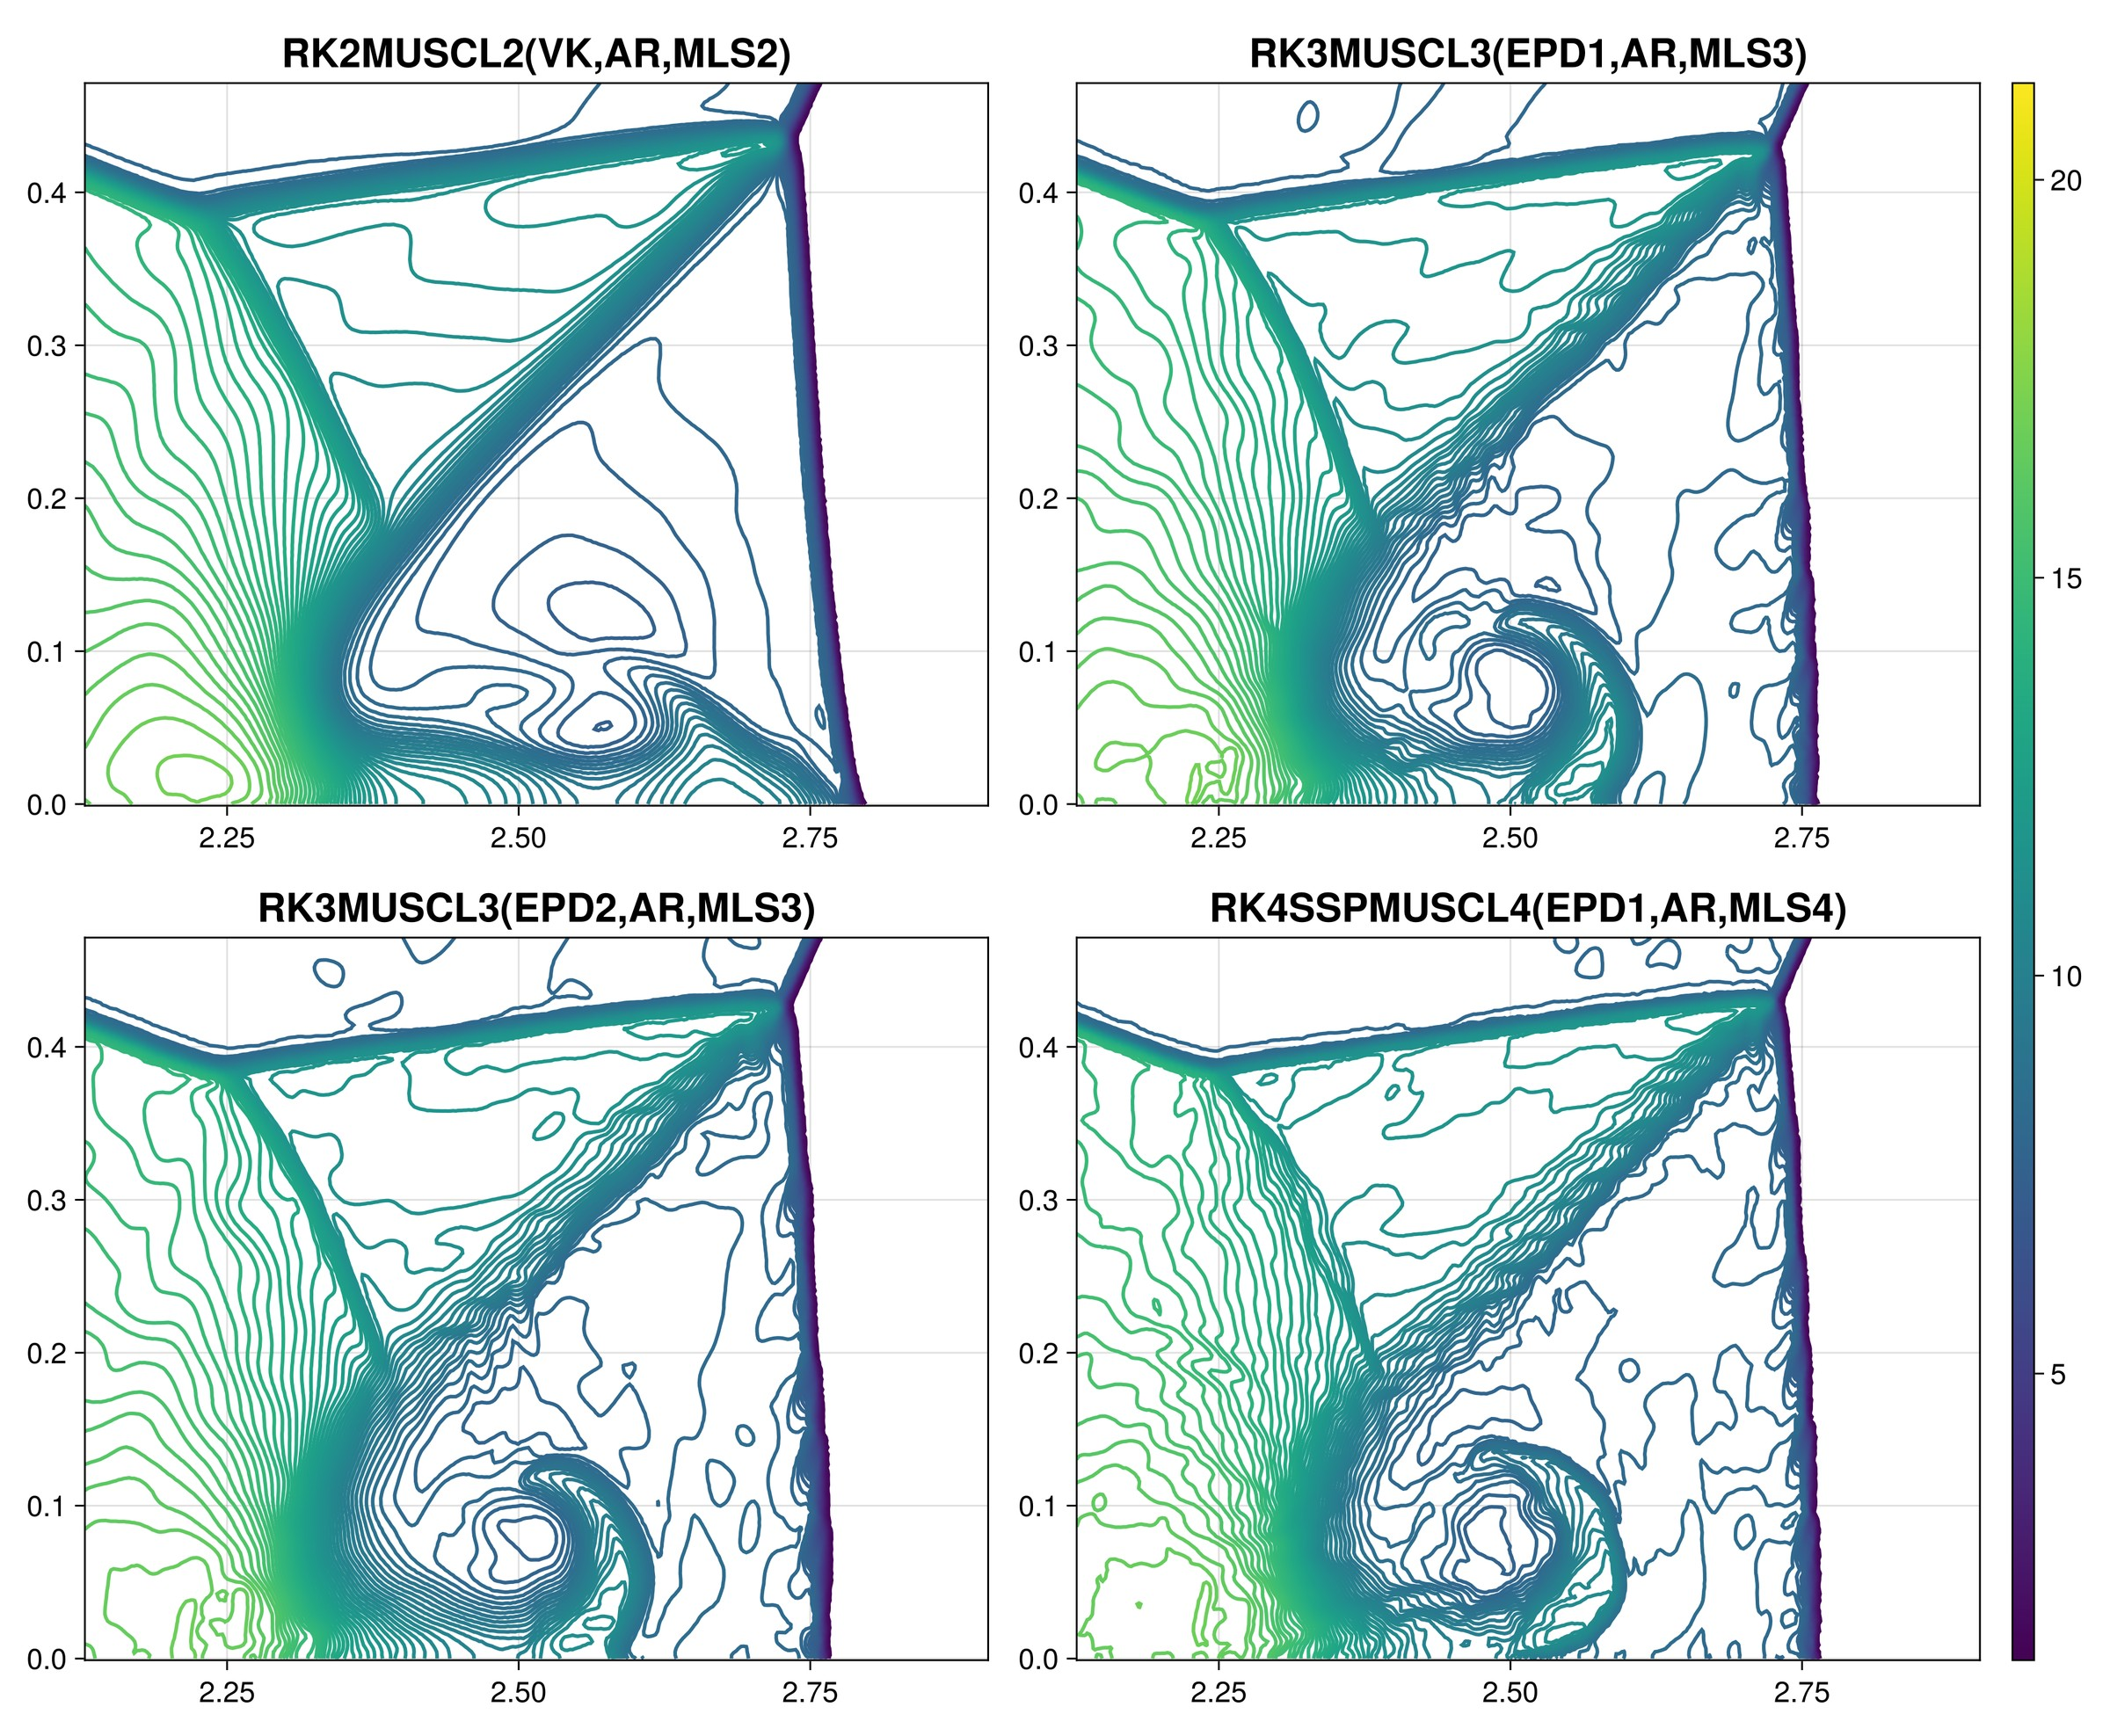
\includegraphics[width=\textwidth]{figures/dmr_zoom_078.jpg}
\caption{Double Mach reflection, detail $[2.13,2.9]\times[0,0.47]$ of \cref{fig:dmr} with $100$ contour levels}\label{fig:dmrzoom}
\end{figure}

\Cref{fig:dmr,fig:dmrzoom} show the density at $t=0.2$. All runs reproduce the characteristic pattern: the incident shock, which meets the top boundary at $x\approx3.05$, its exact position, the reflected shock, the Mach stem, the two triple points, the slip line and the wall jet. The second-order run smears the slip line, and the wall jet forms only a weak curl. The third- and fourth-order runs resolve the slip line sharply, and the jet rolls up into a vortex near $x\approx2.5$, with more structure for $K=4$; the resolution of this roll-up is a common indicator of the numerical dissipation of a scheme. EPD1 and EPD2 give almost the same picture for $K=3$. The stems of the third- and fourth-order runs are almost straight at $x\approx2.76$. In the second-order run the stem bends forward near the wall, to $x\approx2.79$, where the wall jet runs into the foot of the stem. All runs show the highest densities at the wall near $x=\tfrac16$, where the boundary condition switches from the post-shock state to the wall; it is a start-up error caused by the discontinuous boundary data at the foot of the initial shock.

\subsection{Discussion}\label{sec:discussion}

The test problems are demanding even for conservative FV schemes on Cartesian meshes. In the double Mach reflection the resolution of the slip line and of the roll-up of the wall jet is a sensitive measure of numerical dissipation, the discontinuous boundary data at the beginning of the wall cause a start-up error, and Roe's Riemann solver, whose dissipation is low, can produce a kinked Mach stem \cite{Quirk1994}. Our scheme faces these difficulties without the structural advantages of FV methods: it is not exactly conservative (\cref{sec:mass}), its stencils are irregular and overlapping, and its walls are represented by ghost particles with first-order boundary states. Against this background the results are robust. For smooth solutions the schemes attain their design orders up to five on lattices and on perturbed clouds. With the aligned flux every shock computation completes with positive density and pressure, in single precision and without any problem-specific treatment, and with the full derivative degree the third- and fourth-order schemes resolve slip lines and roll-ups markedly better than the second-order scheme.

Three ingredients make the schemes work. First, the derivative degree $\qdiv(k)$ of \eqref{eq:qk} is odd, so that the leading flux errors cancel on symmetric stencils and the truncation error is of order $k$ on lattices (\cref{sec:recfit}); with the even degree $k-1$ the odd orders would lose one order. The parity argument covers symmetric stencils only, but the convergence studies show the same orders on clouds perturbed by $0.2h$ whenever the stencils are large enough for the fits (\cref{sec:smooth}). Second, the aligned orientation of the Rusanov dissipation keeps the first-order fallback positive for derivative weights of any degree. With the geometric orientation, about $40\%$ of the degree-three weights turn the dissipation of a lowered particle into anti-dissipation (\cref{sec:positivity}), so that with this orientation the fallback of the fourth-order scheme with $k_{\mathrm{div}}=4$ is not positive; with the aligned orientation it runs on all shock problems. Third, MOOD checks the forward Euler substeps of the SSP methods, so that every Runge--Kutta stage is a convex combination of checked states (\cref{sec:stagemood}).

The aligned flux removes the trade-off between a positive fallback and conservation. The positivity of the first-order scheme follows from the orientation of the dissipation (\cref{sec:positivity}) instead of the degree of the derivative operator, so the degree can stay the same for all particles, and the pairs of different degrees, whose conservation defect does not decrease under refinement, do not occur. The coupled mode, which keeps these pairs, is positive as well, but it changes the mass by several percent and is not competitive. What remains in the frozen mode is the static asymmetry of the weights on irregular clouds, whose effect decreases under refinement also at moving shocks (\cref{sec:mass}). The price is more dissipation at lowered particles with high-degree weights and, for $k_{\mathrm{div}}\ge3$, a three times smaller time step. The frozen mode with $k_{\mathrm{div}}=K$ keeps the formal order, is positive on all problems and resolves the most structure, at three times the cost of the second-order scheme. With $k_{\mathrm{div}}=2$ the frozen mode costs as much as the second-order scheme and conserves to the floor of all tests, but by \cref{sec:recfit} it is formally of second order in smooth regions, although its reconstructions are of higher degree. The two interface rules trade accuracy for robustness. EPD1 is less dissipative: for $K=3,4$ with $k_{\mathrm{div}}=2$ its Sod errors are $1.6$ to $1.8$ times smaller than those of EPD2, and it keeps the density maximum next to the jet of the Riemann problem, which EPD2 smears; with $k_{\mathrm{div}}=K$ the two rules give almost the same accuracy on the Sod problem and the double Mach reflection. EPD2 is more robust: with $k_{\mathrm{div}}=K$ its minimum pressures are higher on both two-dimensional problems (on the Riemann problem $0.026$ and $0.027$ for $K=3,4$, against $0.018$ and $0.022$ with EPD1), and at $K=4$ its conservation defect at the moving shock decreases under refinement, whereas that of EPD1 stays at about $10^{-3}$ in the range tested.

Limitations are the reduced order of $K=4$ on perturbed clouds with the small radius $\kappa=2.5$ and the first-order ghost-particle boundary conditions. For the present code we recommend the frozen mode with the aligned flux, with $k_{\mathrm{div}}=K$ for the full formal order and $k_{\mathrm{div}}=2$ where cost matters more than the formal order, and MOOD with EPD1 for less dissipation or EPD2 for more robustness.

% ===========================================================================
\section{Open questions and further studies}\label{sec:open}
% ===========================================================================

The experiments raise a number of questions that we leave to future work.
\begin{itemize}
\item \emph{Smooth-extremum detection.} The plateau test and the revised u2 criterion are meant to keep smooth extrema for $K\ge3$; a systematic study on smooth flows is left to future work. Open are a plateau threshold that does not depend on the global range and the resolution, a smooth-extremum test for $K=2$, curvature tests on characteristic or primitive variables, and the behaviour on smooth flows with extrema of several components at once.
\item \emph{Conservation.} With the aligned flux and the frozen degree-one derivative operator the conservation defect decreases under refinement. Constructing antisymmetric face vectors \cite{Chiu2012} would remove it, and constraining the weights to approximately antisymmetric ones \cite{Suchde2017} would reduce it; and with the aligned orientation such weights would keep a positive fallback. It remains open why the frozen mode with $k_{\mathrm{div}}=K\ge4$ and EPD1 keeps defects of about $10^{-3}$ that decrease slowly or not at all (\cref{sec:mass}), and how the defect depends on $h$ in general.
\item \emph{Interface reconstructions.} Lower interface orders truncate the existing fit instead of refitting (\cref{sec:recfit}); whether a refit per interface improves the results at discontinuities, and at what cost, is open; for whole cells, FV-MOOD schemes abandoned truncation for degrees above two \cite[Remark~4]{Diot2012}.
\item \emph{Symmetry of the aligned flux.} On perturbed clouds the two particles of a pair use different fluxes on the pairs whose weights have equal signs (\cref{sec:fluxes}). A symmetric choice, for instance by the sign of $V_ic_{ij}-V_jc_{ji}$, would keep the positivity argument only approximately; whether it improves conservation is open.
\item \emph{Stencils.} The full order of $K=4$ on perturbed clouds with $\kappa=2.5$, and adaptive radii.
\item \emph{Boundary conditions.} Ghost states at reflected positions instead of nearest-donor copies would raise the order at walls.
\item \emph{Further tests.} Refinement studies of the shock problems against converged reference solutions, the Lax and Shu--Osher problems, and three-dimensional problems.
\end{itemize}

% ===========================================================================
\section{Conclusions}\label{sec:conclusion}
% ===========================================================================

We have presented meshfree MUSCL schemes of arbitrary design order for hyperbolic systems on scattered point clouds. Midpoint Riemann problems between MLS reconstructions, combined with an MLS derivative operator with zero row sums, give an update in terms of interface fluxes only. The scheme is exact for polynomial solutions of degree $k-1$ of linear problems, the degree of the derivative operator follows from a parity argument, and the conservation error reduces to the lack of antisymmetry of the volume-weighted derivative weights. A~priori limiters and a stage-wise MOOD procedure with physical and numerical admissibility detection and three interface rules control oscillations. Orienting the Rusanov dissipation by the signs of the derivative weights makes the first-order fallback positive for derivative operators of any degree, so that the derivative degree can stay uniform while MOOD lowers the reconstruction degrees, which removes the pairs of mixed degrees that dominated the conservation error.

The numerical experiments show that these schemes are a promising and robust basis for high-order meshfree computations of compressible flows. For smooth solutions they attain their design orders two to five on lattices and on perturbed clouds. With a derivative operator of degree one the conservation defect at moving shocks decreases under refinement and reaches the resolution of the tests; with higher degrees it is small but, for $K=4$ with EPD1 and for $K=5$, decreases slowly or not at all. On the double Mach reflection and a two-dimensional Riemann problem on perturbed clouds of up to $6.5\times10^5$ particles, all computations complete with positive density and pressure, in single precision, reproduce the characteristic wave patterns without spurious waves apart from start-up errors, and with the full derivative degree the high-order schemes resolve fine structures markedly better than the second-order scheme. Checking the forward Euler substeps of the SSP methods makes every Runge--Kutta stage a convex combination of checked states. The limitations we observed are the reduced order of the fourth-order scheme on perturbed clouds with small stencils and the low-order ghost-particle boundary conditions.

The natural next steps are weights with (approximately) antisymmetric face vectors \cite{Chiu2012,Suchde2017}, and higher-order boundary conditions (\cref{sec:open}). The implementation \cite{jung_hypercloudcore,jung_hypercloud} already supports moving clouds in an arbitrary Lagrangian--Eulerian setting, implicit--explicit time integration, three-dimensional problems and GPUs, which will allow applications to physical problems with a more mature version of the method.

\section*{Software}
The schemes are implemented in HyperCloudCore.jl \cite{jung_hypercloudcore} (version 0.7.8; all results of \cref{sec:experiments}), the test cases are run with HyperCloud.jl \cite{jung_hypercloud} (version 0.5.1), and the figures were produced with PDEStudio \cite{jung_pdestudio} (version 0.4.5). The run configurations and the driver scripts of all experiments are in \cite{jung_meshfree_simulations}.
HyperCloudCore.jl was developed over roughly 18 months with AI assistance whose form changed over the project. In the earlier phase, Gemini models, mostly 3.1 Pro, were used interactively to draft code, explain errors, and suggest implementations, and the first author adapted and integrated this output by hand. From commit 2e4e6fb970 (14.10.2026) onward, most code changes were written with Claude Fable 5.1 in Claude Code, and each change was submitted as a pull request that the first author reviewed manually before merging. Because the two modes were interleaved with the first author's own programming, no precise per-component attribution is given. The correctness of the solver as a whole was established independently of the AI tooling through the convergence studies and benchmarks found in \cref{sec:experiments}. All numerical results in this paper come from executing the code. The full development history is available at \url{https://github.com/industrial-mathematics-group/HyperCloudCore.jl}.

\begin{acknowledgements}
The computations were carried out on the high-performance cluster Elwetritsch of the Regional University Computing Center Kaiserslautern-Landau (RHRZ) at RPTU.
\end{acknowledgements}

% ===========================================================================
% Declarations (Journal of Scientific Computing / Springer Nature): placed
% before the reference list, as required by the submission guidelines.
% ===========================================================================
\section*{Declarations}

\paragraph{Funding}
This work was funded by the Deutsche Forschungsgemeinschaft (DFG, German Research Foundation), grant KL~1105/34.

\paragraph{Competing interests}
\TODO{confirm or replace: The authors have no competing interests to declare that are relevant to the content of this article.}

\paragraph{Ethics approval and consent}
Not applicable.

\paragraph{Data availability}
\begin{sloppypar}% the long repository URL can only break after slashes
The run reports and tables of all computations reported in this paper, the run configurations, the stencil diagnostics and the scripts that produce the wave positions read from the figures are publicly available in the repository \url{https://github.com/industrial-mathematics-group/meshfree-solver-paper} and archived on Zenodo at \TODO{DOI of the Zenodo archive of the repository}.
\end{sloppypar}

\paragraph{Code availability}
The solver HyperCloudCore.jl \cite{jung_hypercloudcore} (version 0.7.8), the simulation framework HyperCloud.jl \cite{jung_hypercloud} (version 0.5.1) and the visualization package PDEStudio \cite{jung_pdestudio} (version 0.4.5) are open source and archived on Zenodo. The run configurations and driver scripts are available in \cite{jung_meshfree_simulations}, and the mathematical addendum \cite{JungAddendum2026} is part of the supplementary material at \url{https://github.com/industrial-mathematics-group/meshfree-solver-paper} (archived at \TODO{DOI of the Zenodo archive of the repository}). A preprint of this paper is available at \url{https://zenodo.org/records/23807966}.

\paragraph{Author contributions}
\TODO{author contribution statement, e.g.\ in CRediT form: Conceptualization: \ldots; Methodology: \ldots; Software: \ldots; Formal analysis and investigation: \ldots; Writing -- original draft preparation: \ldots; Writing -- review and editing: \ldots; Funding acquisition: \ldots; Supervision: \ldots}

\paragraph{Use of large language models}
During the preparation of this work, the first author used Claude Opus 5.5 (Anthropic) to draft substantial parts of the manuscript text. The use of AI tools in the development of the software is described in the section ``Software'' above. The authors reviewed, revised, and verified all content and take full responsibility for the content of this publication. The AI declaration for the supplementary material can be found at \url{https://github.com/industrial-mathematics-group/meshfree-solver-paper}.

% Compact reference list as in the published JSC articles: smaller font,
% no extra space between entries. DOIs stay as full links (JSC guidelines).
\renewcommand{\bibfont}{\small}
\setlength{\bibsep}{0pt plus 0.3ex}
\bibliographystyle{spmpsci}
\bibliography{refs}

\end{document}
